% -------------------------------------------------------------------------------
% Establish page structure & font.
\documentclass[12pt]{report}

\usepackage[total={6.5in, 9in},
	left=1in,
	right=1in,
	top=1in,
	bottom=1in,]{geometry} % Page structure

\usepackage{graphicx} % Required for inserting images
\graphicspath{{images/}} % Any additional images I use (BCU logo, etc) are from here.

\usepackage[utf8]{inputenc} % UTF-8 encoding
\usepackage[T1]{fontenc} % T1 font
\usepackage{float}  % Allows for floats to be positioned using [H], which correctly
                    % positions them relative to their location within my LaTeX code.
\usepackage{subcaption}
\usepackage{amsmath}

% -------------------------------------------------------------------------------
% Declare biblatex with custom Harvard BCU styling for referencing.
\usepackage[
    useprefix=true,
    maxcitenames=2,
    maxbibnames=99,
    style=authoryear,
    dashed=false, 
    natbib=true,
    url=false,
    backend=biber
]{biblatex}

% Additional styling options to ensure Harvard referencing format.
\renewbibmacro*{volume+number+eid}{
    \printfield{volume}
    \setunit*{\addnbspace}
    \printfield{number}
    \setunit{\addcomma\space}
    \printfield{eid}}
\DeclareFieldFormat[article]{number}{\mkbibparens{#1}}

% Declare it as the bibliography source, to be called later via \printbibliography
\addbibresource{Report.bib}

% -------------------------------------------------------------------------------
% To prevent "Chapter N" display for each chapter
\usepackage[compact]{titlesec}
\usepackage{wasysym}
\usepackage{import}

\titlespacing*{\chapter}{0pt}{-2cm}{0.5cm}
\titleformat{\chapter}[display]
{\normalfont\bfseries}{}{0pt}{\Huge}

% -------------------------------------------------------------------------------
% Custom macro to make an un-numbered footnote.

\newcommand\blfootnote[1]{
    \begingroup
    \renewcommand\thefootnote{}\footnote{#1}
    \addtocounter{footnote}{-1}
    \endgroup
}

% -------------------------------------------------------------------------------
% Fancy headers; used to show my name, BCU logo and current chapter for the page.
\usepackage{fancyhdr}
\usepackage{calc}
\pagestyle{fancy}

\setlength\headheight{37pt} % Set custom header height to fit the image.

\renewcommand{\chaptermark}[1]{%
    \markboth{#1}{}} % Include chapter name.


% Lewis Higgins - ID 22133848           [BCU LOGO]                [CHAPTER NAME]
\lhead{Lewis Higgins - ID 22133848~~~~~~~~~~~~~~~
\includegraphics[width=1.75cm]{BCU}}
\fancyhead[R]{\leftmark}

% ------------------------------------------------------------------------------
% Used to add PDF hyperlinks for figures and the contents page.

\usepackage{hyperref}

\hypersetup{
    colorlinks=true,
    linkcolor=black,
    filecolor=magenta,
    urlcolor=blue,
    citecolor=black,
}

% ------------------------------------------------------------------------------
\usepackage{xcolor} 
\usepackage{colortbl}
\usepackage{longtable}
\usepackage{amssymb}
% ------------------------------------------------------------------------------
\usepackage{tcolorbox}
\newcommand{\para}{\vspace{8pt}\noindent}
\usepackage{tikz}
% -------------------------------------------------------------------------------

\title{Using supervised learning for the binary classification of Type 2 Diabetes}
\author{Lewis Higgins - Student ID 22133848}
\date{December 2024}

% -------------------------------------------------------------------------------

\begin{document}


\makeatletter
\begin{titlepage}
    \begin{center}
        
\includegraphics[width=0.7\linewidth]{BCU}\\[4ex]
        {\huge \bfseries  \@title}\\[50ex]
        {\@author}\\[2ex]
        {CMP6202 - Artificial Intelligence \& Machine Learning}\\[2ex]
        {Module Coordinator: Nouh Elmitwally}\\[10ex]
    \end{center}
\end{titlepage}
\makeatother
\thispagestyle{empty}
\newpage


% Page counter trick so that the contents page doesn't increment it.
\setcounter{page}{0}


\tableofcontents
\thispagestyle{empty}

\pagecolor{yellow}
\begin{abstract}
    Probably would benefit from an abstract. You can't really write this until the very end though,
    so return to it then. \textbf{The example work is from a previous year wherein this assessment was a group task.
    You can see that each group member developed one ML model, but you seem to be developing all of them yourself, so don't be mislead
    by the report titles only mentioning one model.}
\end{abstract}
\pagecolor{white}

\chapter{Introduction}

% You've opened by talking about the UK but then transitioned to the whole world?
% Your datasets are American and German in origin, so it's likely that the worldwide perspective will be better.
Diabetes mellitus, or type 2 diabetes, accounts for 90\% of the 4.4 million cases of diabetes in the UK, and it is estimated that 
there are 1.2 million undiagnosed cases of type 2 diabetes across the country \autocite{diabetes_uk_how_nodate}. The rate of type 
2 diabetes per 100,000 individuals is rapidly increasing, with \textcite{khan_epidemiology_2020}'s analysis projecting that by 
2030, the rate will reach 7,079 per 100,000. Many people with diabetes suffer immensely reduced quality of life, with approximately 50\% 
of patients suffering from peripheral neuropathy \autocite{dhanapalaratnam_effect_2024}, an irreversible disability which causes immense pain due 
to nerve damage from high blood sugar \autocite{nhs_peripheral_2022}, which can occur when the patient was unaware they even 
had diabetes. 

\para
Therefore, it is imperative that systems are put in place to enable the swift diagnosis of diabetes, especially type 2 diabetes 
given its major prevalence. This can be accomplished by training machine learning models on existing clinical datasets 
to identify common trends in those with and without type 2 diabetes. This report will document the planning, development 
and evaluation of multiple machine learning models in their classification of whether individuals have type 2 diabetes based 
on multiple clinical factors, specifically through the stages of:

\begin{itemize}
    \item Dataset Identification
    \item Data Integration
    \item Data Preprocessing
    \item Exploratory Data Analysis (EDA)
    \item Model Development 
    \item Model Evaluation
    \item Research Conclusions
\end{itemize}

\pagebreak 
\section{Dataset Identification}

Machine learning models require large amounts of data to train upon, meaning a dataset must be identified consisting of many 
rows and features. This project identified two datasets which could be integrated into one larger dataset, the first of which being 
the well-reputed Pima Indian Diabetes Database \autocite{uci_machine_learning_pima_nodate}, downloaded from \href{https://www.kaggle.com/datasets/uciml/pima-indians-diabetes-database}{Kaggle}, 
a platform for students and researchers alike to download and upload datasets and code for research purposes. The data originates from the National Institute 
of Diabetes and Digestive and Kidney Diseases, who collected this data from Pima Indian\footnote{"Pima Indian" refers to a specific Native American ethnic group rather than people from India.}
women aged 21 and over in hospitals in Phoenix, Arizona, USA, and it has previously seen wide use across academic literature relating to machine learning (\textcite{alzubi_diabetes_2023}, \textcite{zou_construction_2024}, \textcite{joshi_predicting_2021}, \textcite{hayashi_rule_2016}),
where other researchers have also aimed to solve the problem of diabetes classification via supervised learning. This dataset contains 768 rows with 9 features.
% Also cite Kaggle here rather than just hyperlinking it.

\para
This project also includes a second dataset, also from \href{https://www.kaggle.com/datasets/johndasilva/diabetes/data}{Kaggle}, that has been previously used in literature by 
\textcite{zou_construction_2024}. This dataset \autocite{john_dasilva_frankfurt_nodate} is based on data from female patients in Frankfurt, Germany, and includes the same 9 features as the Pima Indian dataset, but includes 2000 rows. By integrating these two datasets into one larger
dataset of 2768 rows, it will be possible to give the machine learning models more data to train upon.

\para Table \ref{tab:Features} details the 9 features seen in both datasets and their descriptions.
% You also need to include their types. Ordinal, nominal, etc as with CMP6230.

\begin{longtable}{ | p{0.3\textwidth} | p{0.5\textwidth} | }
    \hline
    \cellcolor{blue!25}Feature & \cellcolor{blue!25}Description \\
    \hline
    Pregnancies & The number of pregnancies the patient has had. \\
    \hline
    Glucose & Plasma glucose concentration over 2 hours in an oral glucose tolerance test. \\
    \hline
    BloodPressure & Diastolic blood pressure in mm/Hg. \\
    \hline
    SkinThickness & Triceps skin fold thickness (mm) \\
    \hline
    Insulin & 2-hour serum insulin. \\
    \hline
    BMI & Body Mass Index, calculated from the patient's weight and height. \\
    \hline
    DiabetesPedigreeFunction & The product of a function to ascertain the probability of diabetes based on family genetics. \autocite{akmese_diagnosing_2022} \\
    \hline
    Age & The patient's age.\\
    \hline
    Outcome & Whether the patient is likely to develop diabetes.\\
    \hline 
    \caption{The features seen in both datasets.}\label{tab:Features}
\end{longtable}

% An interesting statement was made by Mihai in Week 7.
% He said "You split your data BEFORE EDA to avoid conceptual overfitting".
% This probably should have been considered in the presentation slides.
% The template also is structured in a way where you split before analysis.

\section{Supervised learning task identification}
As previously mentioned, it is possible for patients to have diabetes without knowing. Therefore,
it is paramount that swift and simple diagnosis methods are put in place, which can be achieved 
through the use of supervised learning classification models. This requires the existence of the 
"ground truth", which refers to the label given to data that indicates its class \autocite{c3ai_what_nodate}. 
Within these datasets, the ground truth is present as the 'Outcome' feature, which will be used 
as the target variable for the produced classification models.
% Write more.

% RECALL VERY IMPORTANT DUE TO MEDICAL FIELD!
% SMOTE drawbacks - Synthetic data. Needs data to make more data. In the event of SEVERE imbalance
% (not like your data) it might just give noise instead of useful data.
% KNN + SMOTE - Your dataset is 50% synthetic now. Talk somewhere about the risks of that.
% You removed 98th percentile before imputing your 0s, so was it even the 98th percentile or not?
%   He either didn't notice that or thought it was the right thing to do and didn't mention it so maybe it's fine?
% Split before EDA.
% Why do we do training and testing splits? You were unable to directly answer that during the presentation.

% If you take VSCode screenshots, ensure that your IDE theme is the same across all of them.


\chapter{Exploratory Data Analysis}
This chapter details the EDA processes undertaken with the datasets, including 
key questions that will be answered by the process, as well as the splitting of the 
data into training and testing % and validation
sets.

\section{Data Integration}
% Not included in template but I feel it's necessary to include somewhere because that's what you're doing.
The two datasets must first be merged into one to allow for an overall analysis to be performed.
This is a simple process because they both contain the same 9 features, and is detailed in Figure 
\ref{fig:Integration}.

\begin{figure}[H]
    \centering
    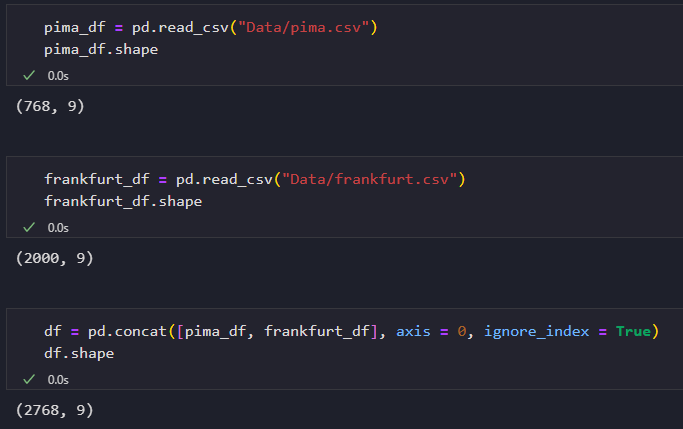
\includegraphics[width=\linewidth]{Integration.png}
    \caption{Integrating the two separate datasets into one larger dataset.}
    \label{fig:Integration}
\end{figure}

\pagebreak 

\section{Question identification and assumptions}
% What questions do you have that thorough EDA would answer?
% Example A gives a good example on what this section should look like.
The key factors involved in the diagnosis of diabetes are critical to understand, which 
can be solved through EDA on these datasets. It is possible to make various assumptions based 
on topical background research of each of the features in the dataset, detailed in Table \ref{tab:Assumptions}

\begin{longtable}{ | p{0.19\textwidth} | p{0.75\textwidth} | }
    \hline
    \cellcolor{blue!25} Feature & \cellcolor{blue!25} Research-based assumptions \\
    \hline
    Pregnancies & Approximately 13.4\% of pregnant women develop a temporary condition known as Gestational 
    Diabetes Mellitus (GDM), which typically subsides after birth \autocite{adam_pregnancy_2023}.
    However, research by \autocite{dennison_absolute_2021} indicates that 33\% of women who develop 
    GDM will go on to develop permanent diabetes mellitus within 15 years. Therefore, it is assumed 
    that pregnancies will positively correlate with the diabetes outcome. It is also expected that 
    pregnancies should naturally positively correlate with age. \\
    \hline
    Glucose & Glucose concentrations are an enormous factor in the diagnosis of diabetes mellitus, being one 
    of the main metrics used to certify the condition, where results over 200mg/dL mean an absolute diagnosis\footnote{The other main metric is insulin deficiency, meaning that the patient could have glucose levels lower than 200mg/dL and still be diagnosed if they are instead insulin deficient. \autocite{aftab_cloud-based_2021}.}
    \autocite{aftab_cloud-based_2021}. It is therefore assumed that the glucose concentrations will be one 
    of the strongest influences of the outcome, and that it will also correlate heavily with insulin levels. \\
    \hline
    BloodPressure & Diastolic blood pressure (DBP) does influence the diagnosis of diabetes mellitus, as 
    56.2\% of recently diagnosed patients presented with elevated DBP in \textcite{nelaj_high_2023}'s limited 
    study of 126 patients, but it is not a decisive factor by itself. Therefore, it is assumed that there will 
    be some correlation between DBP and the outcome, but not as major as other factors like plasma glucose levels.\\
    \hline
    SkinThickness & It is a frequent assumption even non-academically that people who weigh more, and by consequence have higher 
    skin thickness in certain areas such as the triceps, have a higher risk of developing conditions like type 2 diabetes. This is 
    backed by a study by \textcite{ruiz-alejos_skinfold_2020}, which found strong associations between skin thickness and diabetes mellitus,
    as well as high blood pressure. Therefore, it is assumed that there will be a strong correlation between tricep skin thickness and the outcome, 
    as well as an expectation of strong correlations between thickness, BMI and blood pressure.\\
    \hline
    Insulin & Diabetes mellitus is directly associated with insulin deficiency, and as such, it is assumed that this factor will be 
    the strongest influence in the outcome. This is because 2-hour serum insulin tests, as used in this dataset, are frequently 
    part of HOMA-IR\footnote{Homeostasis Model Assessment of Insulin Resistance, used to measure insulin resistance \autocite{tahapary_challenges_2022}, which can be used in both type 1 and type 2 diabetes diagnosis \autocite{khalili_are_2023}.}
    assessments. \\
    \hline
    BMI & BMI is likely to be a significant factor in the outcome, which is backed by previous academic studies indicating that 71\% 
    of studied individuals showed increases in BMI prior to diagnosis \autocite{donnelly_trajectories_2024}. Additionally, BMI is used in insulin resistance measurement assessments,
    which are key assessments in diabetes diagnosis, meaning that it is a safe assumption that BMI will be a large factor in the outcome. \\
    \hline
    DiabetesPedigree- Function & People are more likely to develop diabetes mellitus if there is a family genetic history of the condition, though it is not 
    directly caused by any one particular gene \autocite{diabetes_uk_what_nodate}. With the pedigree function aiming 
    to quantify the inheritance probability, it can be assumed that it will likely correlate heavily with the outcome. \\
    \hline
    Age & \textcite{chackrewarthy_age_2012} studied the effects of age as a risk factor for diabetes mellitus, finding that many natural associated 
    factors of ageing including increases in body fat and decreases in lipid metabolism had considerable influence on the development of insulin 
    resistance and diabetes mellitus by consequence. Therefore, it is likely that there will be a noticeable correlation between a patient's age 
    and the outcome. 
     \\
    \hline
    \caption{Research-based assumptions prior to any EDA.}\label{tab:Assumptions}
\end{longtable}

\para Based on these assumptions, the questions that this EDA process aims to answer are:


\begin{longtable}{ | p{0.05\textwidth} | p{0.85\textwidth} | }
    \hline
    \cellcolor{blue!25} ID & \cellcolor{blue!25} Research-based assumptions \\
    \hline
    1 & Are there any missing values or values that are not physically possible?\\
    \hline
    2 & Are there any significant outliers?\\
    \hline 
    3 & Is the dataset evenly balanced in terms of the outcome? If not, what should be done?\\
    \hline 
    4 & Does the rate of diabetes positively correlate with the amount of pregnancies a woman has had?\\
    \hline
    5 & Does the amount of pregnancies influence any of the other features?\\
    \hline
    6 & What is the distribution of blood glucose levels in patients with and without diabetes?\\
    \hline
    7 & Does BMI influence glucose levels?\\
    \hline
    8 & Is diastolic blood pressure a worthwhile diagnosis method in this dataset?\\
    \hline
    9 & Is the average skin thickness of those with diabetes actually higher than those without?\\
    \hline
    10 & How does the relationship between insulin and glucose change between those with and without diabetes?\\
    \hline
    \caption{The questions that this EDA process aims to answer.}\label{tab:Questions}
\end{longtable}

\section{Splitting the dataset}
% How was the data split?
% Why do we split? Why 80:20 as you're doing?
% Train/test? KFold?
% Maybe do train/test at first and KFold in an iterative improvement and compare the models?
% Training and testing sets are a minimum. It's possible they also want a VALIDATION set
It is good practice to first split the data into training and testing sets before performing exploratory data analysis
to avoid conceptual overfitting, also known as data leakage. Conceptual overfitting occurs when insights gained from the entire dataset 
influence model development decisions, which may eventually lead to actual overfitting. By excluding the training data from the analysis,
it effectively simulates a real-world environment where the data being given to the model is not known, even to its developers.

% !!! Give a better and longer definition of overfitting.

\para Splitting the data is a mandatory process when developing supervised learning models, primarily for the prevention of overfitting.
Overfitting is a significant challenge in machine learning, where models can perform exceptionally well on their original training data but 
are unable to generalize to unseen data, making them unsuitable for deployed use. The training set must consist of a large portion of the 
data so that the model has enough information to analyse and discover trends within, whereas the testing set is a smaller, unseen remainder 
of the data that the model's predictions can be evaluated against using various metrics. A key point of determination is the proportions 
of the dataset that should go in each set - there is no 'one-size-fits-all' percentage that can provide the best results for every possible dataset \autocite{sivakumar_trade-off_2024},
and factors such as the size of the dataset play a large part in this. Most commonly, splits are either 70:30 or 80:20 for training and testing sets 
respectively.

\para The integrated dataset for this project is 2,768 rows. This is considered to be a small dataset, and as such, it will be best to 
maximize the size of the training split, so a split of 80\% training and 20\% testing was used, visualized in Figure \ref{fig:TrainTestDiagram}.

\begin{figure}[H]
    \centering
    \begin{tikzpicture}[
        full/.style={draw, rectangle, minimum width=10cm, minimum height=1.5cm, fill = lightgray},
        train/.style={draw, rectangle, minimum width=8cm, minimum height=1.5cm, fill = cyan},
        test/.style={draw, rectangle, minimum width=2cm, minimum height=1.5cm, fill = pink},
        arrow/.style={<->, thick}
    ]
    
    % Full dataset block
    \node[full] (full) at (0,1.5) {Full dataset (2768 rows)};
    
    % Training set block
    \node[train] (train) at (-1,0) {Training};
    
    % Testing set block
    \node[test] (test) at (4, 0) {Testing};

    % Proportion indicators
    \draw[arrow] (-5,-1.2) -- (2.9,-1.2) node[midway, below] {80\%};
    \draw[arrow] (3.1,-1.2) -- (4.9,-1.2) node[midway, below] {20\%};
    
    \end{tikzpicture}
    \caption{A visual representation of the train/test split.}
    \label{fig:TrainTestDiagram}
\end{figure}

\para To accomplish this, the data must first be split into $X$ and $y$ tables, where $X$ consists of the eight features, and $y$ is the target variable.
After the data is split to $X$ and $y$, it can be split into training and testing sets through Scikit-Learn's "train\_test\_split" method, as depicted in Figure \ref{fig:TrainTestSplit}

\begin{figure}[H]
    \centering
    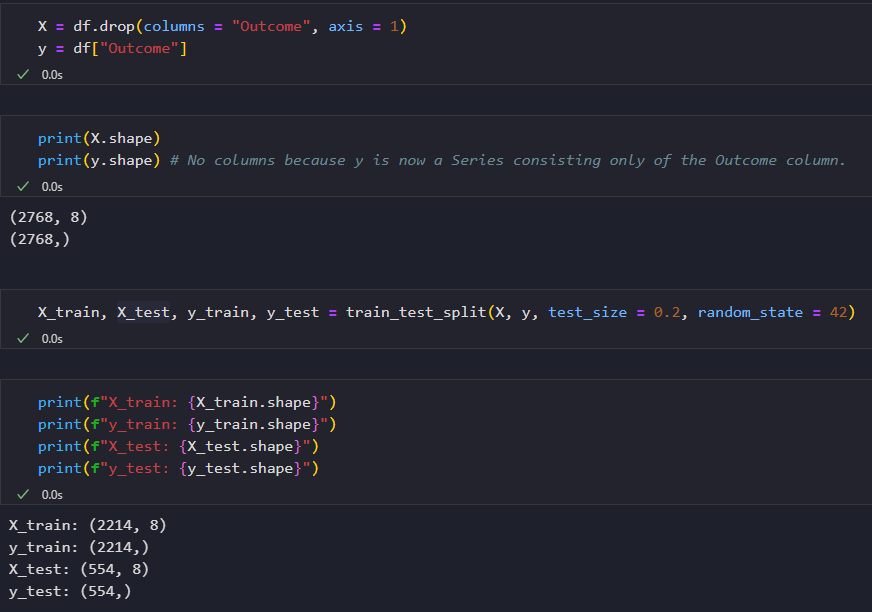
\includegraphics[width=\linewidth]{EDA/TrainTestSplit.png}
    \caption{Splitting the data at an 80:20 ratio.}
    \label{fig:TrainTestSplit}
\end{figure}

\para By default, this method will first shuffle all rows in the dataset before splitting it, which introduces an element of randomness which can damage 
reproducibility. To combat this, the "random\_state" parameter can be set to ensure that the same shuffle will occur every time.

\para When performing EDA, the Outcome column will be necessary to the analysis, so a deep copy\footnote{A complete copy rather than a pointer to the original data}
of X\_train was made with y\_train (the Outcome column) being added to it, merging the two back into a full training set, shown in Figure \ref{fig:FullTrainingSet}.

\begin{figure}[H]
    \centering
    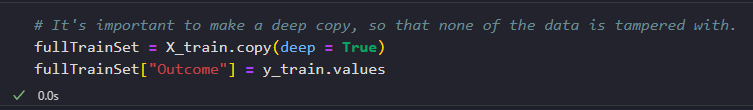
\includegraphics[width=\linewidth]{EDA/FullTrainingSet.png}
    \caption{Duplicating X\_train and adding the Outcome column for EDA.}
    \label{fig:FullTrainingSet}
\end{figure}


\section{EDA process and results}
In the interest of report conciseness, the full EDA process and results accompany this report as Appendix A. They were performed using the Seaborn Python library,
which uses Matplotlib to produce convenient visualisations to answer each question posed in Table \ref{tab:Questions}. The topics and issues identified
during the process are solved in Section \ref{sec:Preprocessing}.


\section{EDA conclusions}
The extensive EDA conducted in Appendix A provided clear answers to each question posed in Table \ref{tab:Questions}, 
which are detailed below in Table \ref{tab:Answers}.

\begin{longtable}{ | p{0.05\textwidth} | p{0.85\textwidth} | }
    \hline
    \cellcolor{blue!25} ID & \cellcolor{blue!25} EDA-based answer \\
    \hline
    1 & There are missing values in the dataset that were not originally presented as such; they were instead
    0s in columns where this would be physically impossible. After converting the impossible 0s to missing values 
    with NumPy, it was established that there were 18 missing Glucose values, 125 missing BloodPressure values,
    800 missing SkinThickness values, 1330 missing Insulin values, and 39 missing BMI values.
    % \begin{itemize}
    %     \item 18 missing Glucose values.
    %     \item 125 missing BloodPressure values.
    %     \item 800 missing SkinThickness values.
    %     \item 1330 missing Insulin values.
    %     \item 39 missing BMI values.
    % \end{itemize}
    \\
    \hline
    2 & The analysis identified significant outliers across various features using box plots. 
    Particularly extremely outliers were noted in the SkinThickness, BMI, and Insulin columns. These outliers
    could affect data scaling and model performance, and will need to be transformed in data cleaning. \\
    \hline 
    3 & The dataset is imbalanced, with 65.5\% of rows in the training set having an outcome of 0, while the remaining 
    35.5\% had an outcome of 1.\\
    \hline 
    4 & The EDA did show a somewhat positive correlation between the number of pregnancies and diabetes outcomes, 
    although pregnancies alone are not decisive in predicting diabetes.\\
    \hline
    5 & Pregnancies are found to correlate with age, as expected, but do not significantly influence other features.\\
    \hline
    6 & There is a clear and significant distinction in glucose levels between diabetic and non-diabetic individuals,
    with higher levels being mostly present in those with diabetes, making it a strong indicator.\\
    \hline
    7 & A slight positive correlation is observed between BMI and glucose levels, indicating that higher BMI could be 
    associated with higher glucose levels.\\
    \hline
    8 & Blood pressure shows some correlation with diabetes outcomes but is not a strong standalone diagnostic factor. 
    However, like pregnancies, previously mentioned academic research specifies that it is still a useful feature to keep.\\
    \hline
    9 & Individuals with diabetes tend to have higher skin thickness on average, although this feature contains significant high outliers
    in both individuals with and without diabetes.\\
    \hline
    10 &  The relationship between insulin and glucose varies between diabetic and non-diabetic individuals, with diabetic individuals 
    showing higher glucose levels as a result of lower insulin levels, which is expected of type 2 diabetes.\\
    \hline
    \caption{Answers to the questions after the completion of the EDA process.}\label{tab:Answers}
\end{longtable}

\pagebreak
\para Overall, the EDA process conducted in Appendix A has been highly beneficial for many reasons. Firstly, it identified critical data issues, 
such as the abundance of missing values and outliers, which are essential to address to improve model accuracy and reliability. By recognizing these 
issues early, the EDA ensures that data preprocessing steps can be effectively planned to mitigate their impact. Secondly, the EDA highlighted significant
correlations between features and the diabetes outcome, such as the strong influence of glucose levels and BMI on diabetes diagnosis. Understanding these
relationships helps in feature selection and engineering, which are crucial for building effective predictive models. Additionally, the EDA revealed class 
imbalances in the dataset, guiding the development of strategies to handle this imbalance during model training to prevent biased predictions. 

\para The insights gained from the EDA therefore provide a solid foundation for informed decision-making in the experimental design and model development, 
ensuring that the models are trained on clean, balanced, and relevant data, ultimately enhancing their predictive performance. This is especially crucial 
given that the models would be used in the medical field, where incorrect predictions could have life-changing ramifications.

\chapter{Experimental Design} % This may benefit from being its own .TeX file.
This chapter details the planned algorithms to be leveraged against this dataset,
as well as the metrics to evaluate them. Furthermore, leveraged data preprocessing techniques
are deeply explored, as well as some potential limitations relating to their use.

\section{Identification of chosen algorithms}\label{sec:ChosenAlgorithms}
% What algorithms? 
% Why those? 
% How do those algorithms work?
Five classification algorithms will be leveraged on this dataset, these being Random Forests,
Support Vector Machines, Logistic Regression, Na\"ive Bayes, and K-Nearest Neighbours. These were 
selected due to their previous use in literature based on these datasets, and also due to their 
high prevalence across many fields. Detailed descriptions of each algorithm, including their 
mathematical formulae, can be found in Appendix B - Classification Algorithms.

\section{Identification of appropriate evaluation techniques}
% What metrics?
% Why those?
% How do they show the model's performance?
When evaluating classification models, it is crucial to select appropriate metrics that provide a comprehensive understanding of the model's performance.
For this project, three key evaluation metrics will be used: accuracy, recall, and F1 score. 
By using these three metrics in combination, we can gain a comprehensive understanding of our classification models' performance. Accuracy provides an overall measure of correctness,
recall ensures positive cases are not missed, and the F1 score offers a balanced view that accounts for both precision and recall.
This multi-metric approach will allow for a detailed evaluation of the five models.

\subsection{Accuracy}
Accuracy is the most straightforward metric, measuring the overall correctness of the model's predictions. It is calculated as the ratio of correct predictions
(both true positives [TP] and true negatives [TN]) to the total number of predictions, including false positives [FP] and negatives [FN] \autocite{google_classification_nodate},
shown in Equation \ref{eq:Accuracy}.

\begin{equation}\label{eq:Accuracy}
    \text{Accuracy} = \frac{\text{TP} + \text{TN}}{\text{TP} + \text{TN} + \text{FP} + \text{FN}}
\end{equation}


\para While accuracy is intuitive and easy to interpret, it can be misleading in cases
of imbalanced datasets, which is a concern in this dataset that will need to be addressed in preprocessing.

\subsection{Recall}
Recall, also known as sensitivity or true positive rate, is particularly important in medical diagnosis scenarios like diabetes detection. It measures
the model's ability to correctly identify all positive cases. In this context, high recall ensures that we minimize the number of diabetic patients
who are incorrectly classified as non-diabetic (false negatives). This is crucial because missing a diabetes diagnosis could have serious health implications for the patient such 
as neuropathy, vision problems and other health complications such as heart disease or strokes \autocite{nhs_type_nodate}.

\begin{equation}\label{eq:Recall}
    \text{Recall} = \frac{\text{TP}}{\text{TP} + \text{FN}}
\end{equation}

\subsection{F1 Score}
The F1 score provides a balanced measure of the model's performance by combining precision\footnote{The rate of correctly classified positives. Often has an inverse relationship with Recall \autocite{google_classification_nodate}.}
and recall into a single metric, and is particularly useful with imbalanced datasets such as the one used in this project.
The F1 score is calculated as the harmonic mean\footnote{The reciprocal of the mean of the reciprocals of the features. A reciprocal is 1 divided by the number, such as 4's reciprocal being 1/4.}
of precision and recall, giving equal weight to both metrics, which is useful because in a medical context, false positives and negatives are extremely important 
and can bear significant consequences.

\begin{equation}\label{eq:Precision}
    \text{Precision} = \frac{\text{TP}}{\text{TP} + \text{FP}}
\end{equation}

\begin{equation}\label{eq:F1Score}
    \text{F1-Score} = 2 \times \frac{\text{Precision} \times \text{Recall}}{\text{Precision} + \text{Recall}}
\end{equation}



\section{Data Cleaning and Pre-processing Transformations}\label{sec:Preprocessing}
% How have you handled missing data? KNN Imputation as Zou et al. did because mean and median were catastrophic.

% SCALING - STANDARDSCALER THEN ROBUST IN ITERATIVE IMPROVEMENT?
% SMOTE AND NO SMOTE IN ITERATIVE IMPROVEMENT?

% Significant problem: KNN Imputation of the testing set is not optimal as you're technically then testing the model
% on data it's already been trained on. Consider alternative improvement - mean imputation for testing set after KNN
% applied to train? If this works, it's an iterative improvement.
\subsection{Data encoding}
Data encoding was not necessary in this dataset as all features were already numeric. However, a detailed description of typical 
encoding processes can be found in Appendix C.

\subsection{Data cleaning}
The EDA revealed the necessity for data cleaning in this dataset through the transformation of outliers and imputation of missing values.

\subsubsection{Outlier handling}
It was observed that all columns had outliers, with some having particularly extreme outliers that caused massive skew in the data and 
the visualisations produced from it. To address these, data was constrained to be within the 1st and 99th percentiles, and any data outside 
of these would be increased or decreased to one of these boundaries.

\begin{figure}[H]
    \centering
    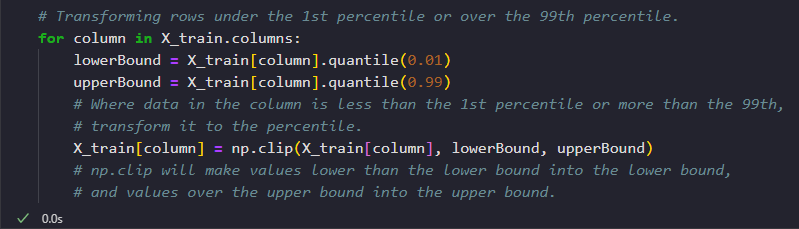
\includegraphics[width=\linewidth]{Preprocessing/OutlierConstraining.png}
    \caption{Using np.clip to transform values less than or greater than the 1st and 99th percentiles.}
    \label{fig:OutlierConstraining}
\end{figure}

\pagebreak 

\subsubsection{Missing data imputation}
After handling the outliers in the data, missing data can be imputed. The selected method for this was KNN imputation,
which uses the KNN algorithm to aggregate data from the $k$ nearest data points and imputes the average of these points 
in place of the missing value \autocite{trainindata_knn_2024}. This method can be very useful as it will not impute many rows 
of the same number as mean or median imputation would do, and instead imputes reasonable values based on similar rows,
which is especially beneficial given the high correlations between some of the missing data (such as Insulin) and data 
that is mostly present (such as Glucose).

\begin{figure}[H]
    \centering
    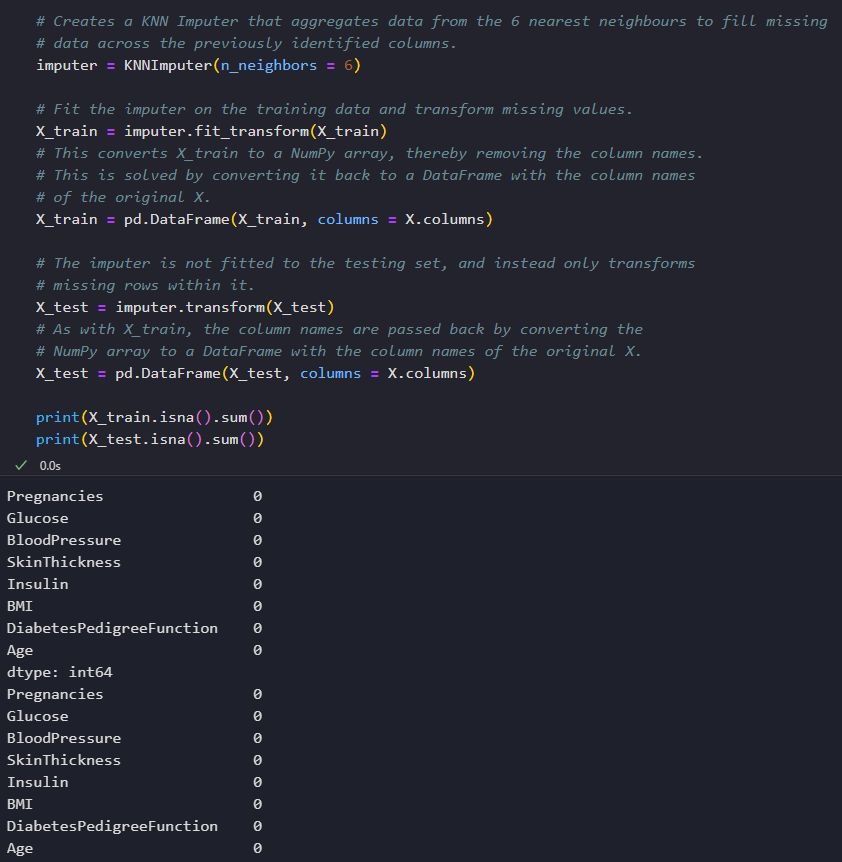
\includegraphics[width=.8\linewidth]{Preprocessing/KNNImputation.png}
    \caption{Using KNN imputation to resolve missing data.}
    \label{fig:KNNImputation}
\end{figure}

\para K was set to 6 in the imputer to increase the amount of data each imputed point is based on, but also to not average 
too many data points, as the data still varies despite containing many less outliers. 
% Bad description, scrap entirely? 6 was chosen randomly, maybe you could go way higher now with outlier removal.

\subsection{Data scaling}
After imputing missing data, scaling can occur. Algorithms such as KNN and SVMs rely heavily on the distance 
between data points, meaning they can be heavily skewed by large distances between real numbers. Due to the high 
variance in the dataset as many features use different scales (Age, Insulin, SkinThickness, and BMI for example), 
it was decided that standardisation will be the scaling procedure. Standardisation uses the formula in Equation \ref{eq:Standardisation}
to scale data so that it has a mean of 0 and a standard deviation of 1.

\begin{equation}\label{eq:Standardisation}
    Z = \frac{X - \mu}{\sigma}
\end{equation}
\begin{align*}
    Z & \text{ is the standardized value (also known as "z-score")} \\
    X & \text{ is the original value of the feature} \\
    \mu & \text{ is the mean of the feature} \\
    \sigma & \text{ is the standard deviation of the feature}
\end{align*}

\begin{figure}[H]
    \centering
    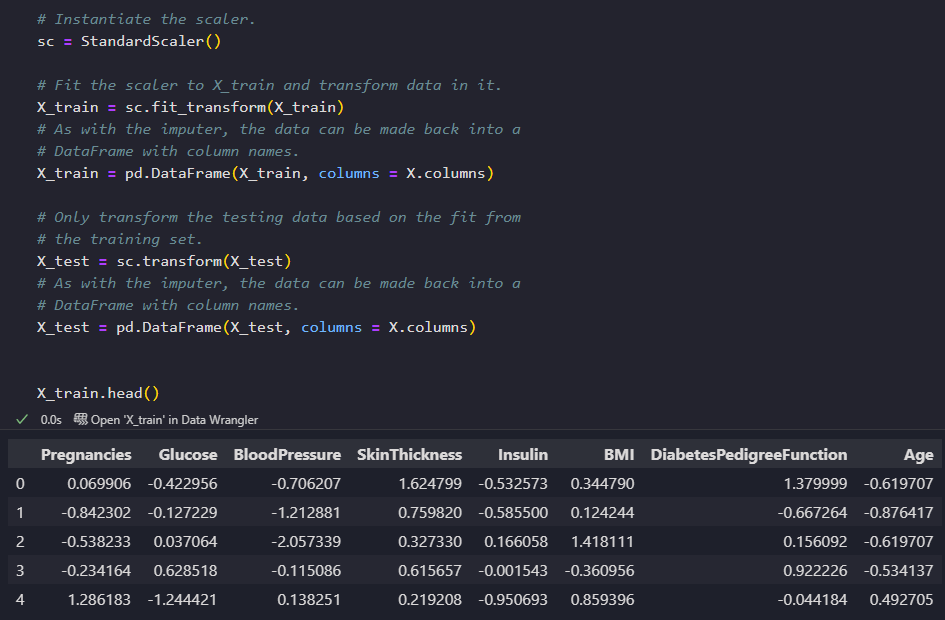
\includegraphics[width=\linewidth]{Preprocessing/Standardisation.png}
    \caption{Using a StandardScaler to standardise the data.}
    \label{fig:Standardisation}
\end{figure}

\pagebreak

\subsection{Data balancing}
It was also established during EDA that the dataset is imbalanced, mostly containing rows without diabetes. Therefore,
the Synthetic Minority Oversampling Technique (SMOTE) was used to generate synthetic data to balance the classes. 
SMOTE also uses the KNN algorithm to generate data, but randomly selects nearest neighbours and generates data in-between
the selected sample and the neighbour \autocite{trainindata_overcoming_2023}. This is repeated until the classes are balanced.

\begin{figure}[H]
    \centering
    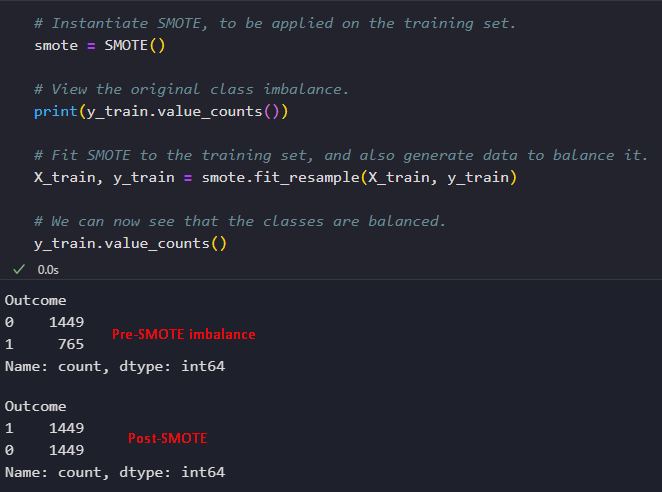
\includegraphics[width=.8\linewidth]{Preprocessing/SMOTE.png}
    \caption{Using SMOTE to balance the training set.}
    \label{fig:SMOTE}
\end{figure}

\para SMOTE is not used to balance the testing set, as the testing set should be exclusively real data
so that an accurate representation of the model's ability to predict real data can be gathered \autocite{ozbun_properly_2021}.



\section{Limitations and Options}
% What are the limitations of this approach?
%   The sheer amount of missing insulin data and imputation means the datasets are basically synthetic now.
A key limitation in this design comes from the datasets themselves; they contain colossal amounts of missing data, 
with almost half of the Insulin values missing. With Insulin being such an integral part of type 2 diabetes diagnosis,
the issue of having so much missing data cannot be overlooked. While it was addressed using KNN imputation, the synthetic 
data generated by this approach could possibly be of poor quality.

\para Furthermore, SMOTE was used to balance the classes. While SMOTE is a useful tool, it can introduce noise to a dataset.
Additionally, SMOTE was performed after the KNN imputation, meaning that a substantial amount of the dataset was then synthetic data.

\para In future projects, it would be best to use more organised and clean datasets, where such substantial 
preprocessing measures would not be necessary. Furthermore, the features in the dataset are all numerical.
While this is good for the development of machine learning models, it did not allow for the demonstration 
of encoding techniques, which were instead described in Appendix C.

\chapter{Model Development} % Titled "predictive modelling / model development" in template.
% This may benefit from being its own .TeX file.
This chapter details the training and evaluation processes of the original produced models
before any iterative improvements such as hyperparameter tuning.

% 3929 without appendices, 6417 with.

% EDA - SHOW DATA DISTRIBUTIONS TO ADD CREDENCE TO YOUR POINT MADE IN DATA SCALING.

\section{Predictive modelling process}
% What processes did you undertake to train the models?
%   How did you use the pre-processed data for training?
%   What parameters did you use?
%   Screenshots of code or Minted code blocks necessary.

\section{Results on seen data}
% Discuss evaluating your model on previously seen data i.e. the training set.
% Screenshots of code or Minted code blocks necessary.

% For Random Forest, you may be able to use "export_graphviz" to show the conditions of the decision tree itself.

\chapter{Evaluation and further improvements}
This chapter details the extensive evaluation of each model, as well as iterative improvements 
that were made to enhance their performance.
% No idea what this section entails, as the template is quite non-descript on it. (or over-descript idk)
% I believe it's about the iterative improvements to the models?
% You should talk about GridSearchCV and how it allowed for optimal hyperparameter tuning.

% (The secret was primarily to increase KNN imputer's neighbours. Increased all metrics obscenely.)

\chapter{Conclusion}
% THIS IS NOT A DRAFT. YOU NEED TO PROOFREAD THIS!
% ENSURE IT'S STRUCTURED WELL WITH NO WEIRD PAGE BREAKS.

% You say "will be" a lot, but a report is past tense. Change these to "is".

% Upon reaching this point, go back and make sure your introduction is still valid and makes sense in relation
% to the rest of the document. This was an issue in CMP6230 that you caught last-minute.

% Pay significant attention to the conclusion, especially the individual learning reflection, as Nouh mentioned 
% in previous weeks that he's starting his reading from there and it's a heavy bearing on your grade (10% so 8% overall)

% A few times across the report you mention "the 9 features". I don't think the target variable is a feature, so shouldn't it be
% the 8 features?

\section{Summary of results} 
% You've done this in labs, make a DF of all models and accuracies, plot it on a graph.
% Discuss the evaluation results for your final models.
% Summarise the entire report:
%   The problem
%   The datasets
%   Your methodology
%   Your results
%   Any insights gained?

\section{Reflection on Individual Learning}
% Nouh has previously stated he will begin here. This section could be 10% of the marks.
% What did you learn by doing this assignment?
% What aspects of the assignment did you enjoy most?
% How will you further hone your skills in future?


% You need evidence for this section. Miscellaneous certificates as well as public Github repositories.
% On that topic, many of your repos aren't exactly "sanitised" for public viewing and had many colorful notes in
% that were only meant to be read by you. Pick and choose repos that are fine.
% DataVis is theoretically fine, but the commit history contains many wonderful messages I'd rather weren't seen.

% This section alone is about 300 words. Cutting it down could be best.
Over the course of this module and others, I have enhanced my skills with a wide variety of tech stacks to a degree 
I previously thought impossible. I have thoroughly enjoyed expanding my Python skills for data science and machine learning 
with the use of industry standard packages like Pandas and NumPy. This project in particular has heavily challenged me, 
requiring extensive research into many academic papers and web resources to further my knowledge of the medical field 
and machine learning trends.

\para I have always enjoyed writing code from as young as 11 years old. I originally began by creating games on the Roblox platform 
using their specialised fork of the Lua language, and expanded beyond that into Python as I furthered my knowledge of computing 
and IT. Also, I have a \href{https://github.com/LewGoesB00M}{personal GitHub account}, which I use for version control and iterative 
saving of my University work, including for this module in the \href{https://github.com/LewGoesB00M/CMP6202}{CMP6202 repository}, 
where every step taken in the production of this report is documented across many commits.

\para Irrespective of my personal appreciation and enjoyment in writing code, the particular topic of this project was one 
that is close to my heart - members of my family suffer from type 2 diabetes and other health complications that arose from it,
including neuropathy (intense pain and/or weakness), retinopathy (loss of vision) and even heart attacks and strokes. 
Therefore, I am intensely interested in the applications of my passions in AI and Machine Learning to make a positive difference 
for others, and I believe that the knowledge I have gained through this project will be a strong asset in doing so.

% When you're done and get back to here, write the abstract!

% Interesting trick to instead make the chapter number the letter A for this appendix.
\begingroup
\renewcommand\thechapter{A}
\titleformat{\chapter}[display]
{\normalfont\huge\bfseries}{}{20pt}{\Huge}
\setcounter{section}{0} % Set the section counter back to 0 so the conclusion doesn't interfere.

\chapter*{Appendix A - EDA Process and Results}
\addcontentsline{toc}{chapter}{Appendix A - EDA Process and Results}
\markboth{Appendix A}{}
Problems identified through the EDA conducted in this Appendix were resolved in Section \ref{sec:Preprocessing}.

\section{Identification of missing or impossible values}
An initial glance at the dataset would make it appear as though as there are not any missing values in the dataset, as shown in Figure \ref{fig:InitialNoNAs}.

\begin{figure}[H]
    \centering
    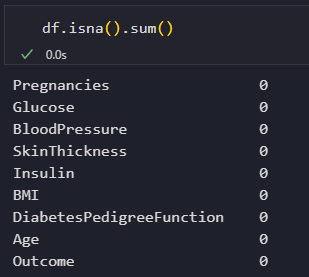
\includegraphics[width=.5\linewidth]{EDA/InitialNoNAs.png}
    \caption{An initial count of missing values before any further analysis.}
    \label{fig:InitialNoNAs}
\end{figure}

\para This would be very good - if it were true. Instead of missing values, this dataset contains impossible values in five columns, highlighted in red in 
Figure \ref{fig:ImpossibleValues}.\footnote{The mean of the outcome is highlighted in blue, as the fact that it is under 0.5 indicates that there are more 
cases of outcome 0 (no diabetes) than 1 (diabetes). This will be further analysed in Section \ref{ASec:Imbalance}.}

\begin{figure}[H]
    \centering
    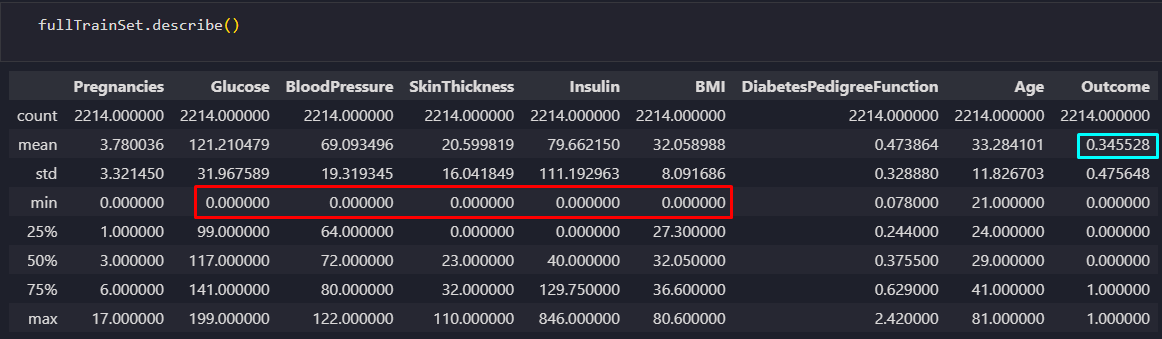
\includegraphics[width=\linewidth]{EDA/ImpossibleValues.png}
    \caption{The overall dataset description. Physically impossible values are \textcolor{red}{in red}.}
    \label{fig:ImpossibleValues}
\end{figure}

\pagebreak
\para It is not possible for a living person to have a 0 in any of the five highlighted columns, and these datasets do not contain information of the deceased.
Therefore, it can be deduced that these values are erroneous, and should be treated as though they are missing. It is theorised by some in Kaggle discussions of these 
datasets that the zeroes in the Insulin column actually meant "imperceptible levels", which would have been useful data. However, a further review of literature around the datasets,
especially \textcite{hayashi_rule_2016}'s paper, led to the discovery that these zeroes truly are missing values that were missing due to experimental invalidity at the time 
of their collection.

\begin{figure}[H]
    \centering
    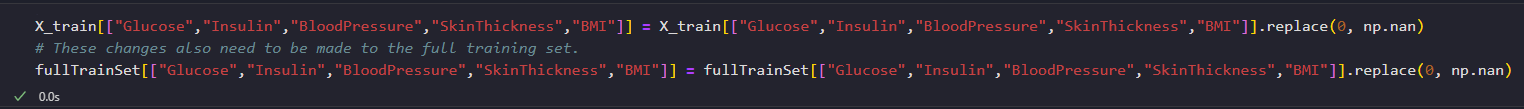
\includegraphics[width=\linewidth]{EDA/ConvertImpossibleValues.png} 
    \caption{Converting the impossible values to NaNs which are recognised by Pandas.}
    \label{fig:ConvertImpossibleValues}
\end{figure}

\para This conversion is applied to the actual X\_train set for model training, as well as to the fullTrainSet copy made in Figure \ref{fig:FullTrainingSet}.
Also, it is assumed that there will also be impossible values in the testing set, so they are also converted to NaNs there.
Now that there are officially recognised missing values, they can be visualised using the Missingno package, which can produce a 
matrix of missing values by column, seen in Figure \ref{fig:MissingnoMatrix}.
% bar chart of the amount of values in each column, seen in Figure \ref{fig:MissingnoBar}.

\begin{figure}[H]
    \centering
    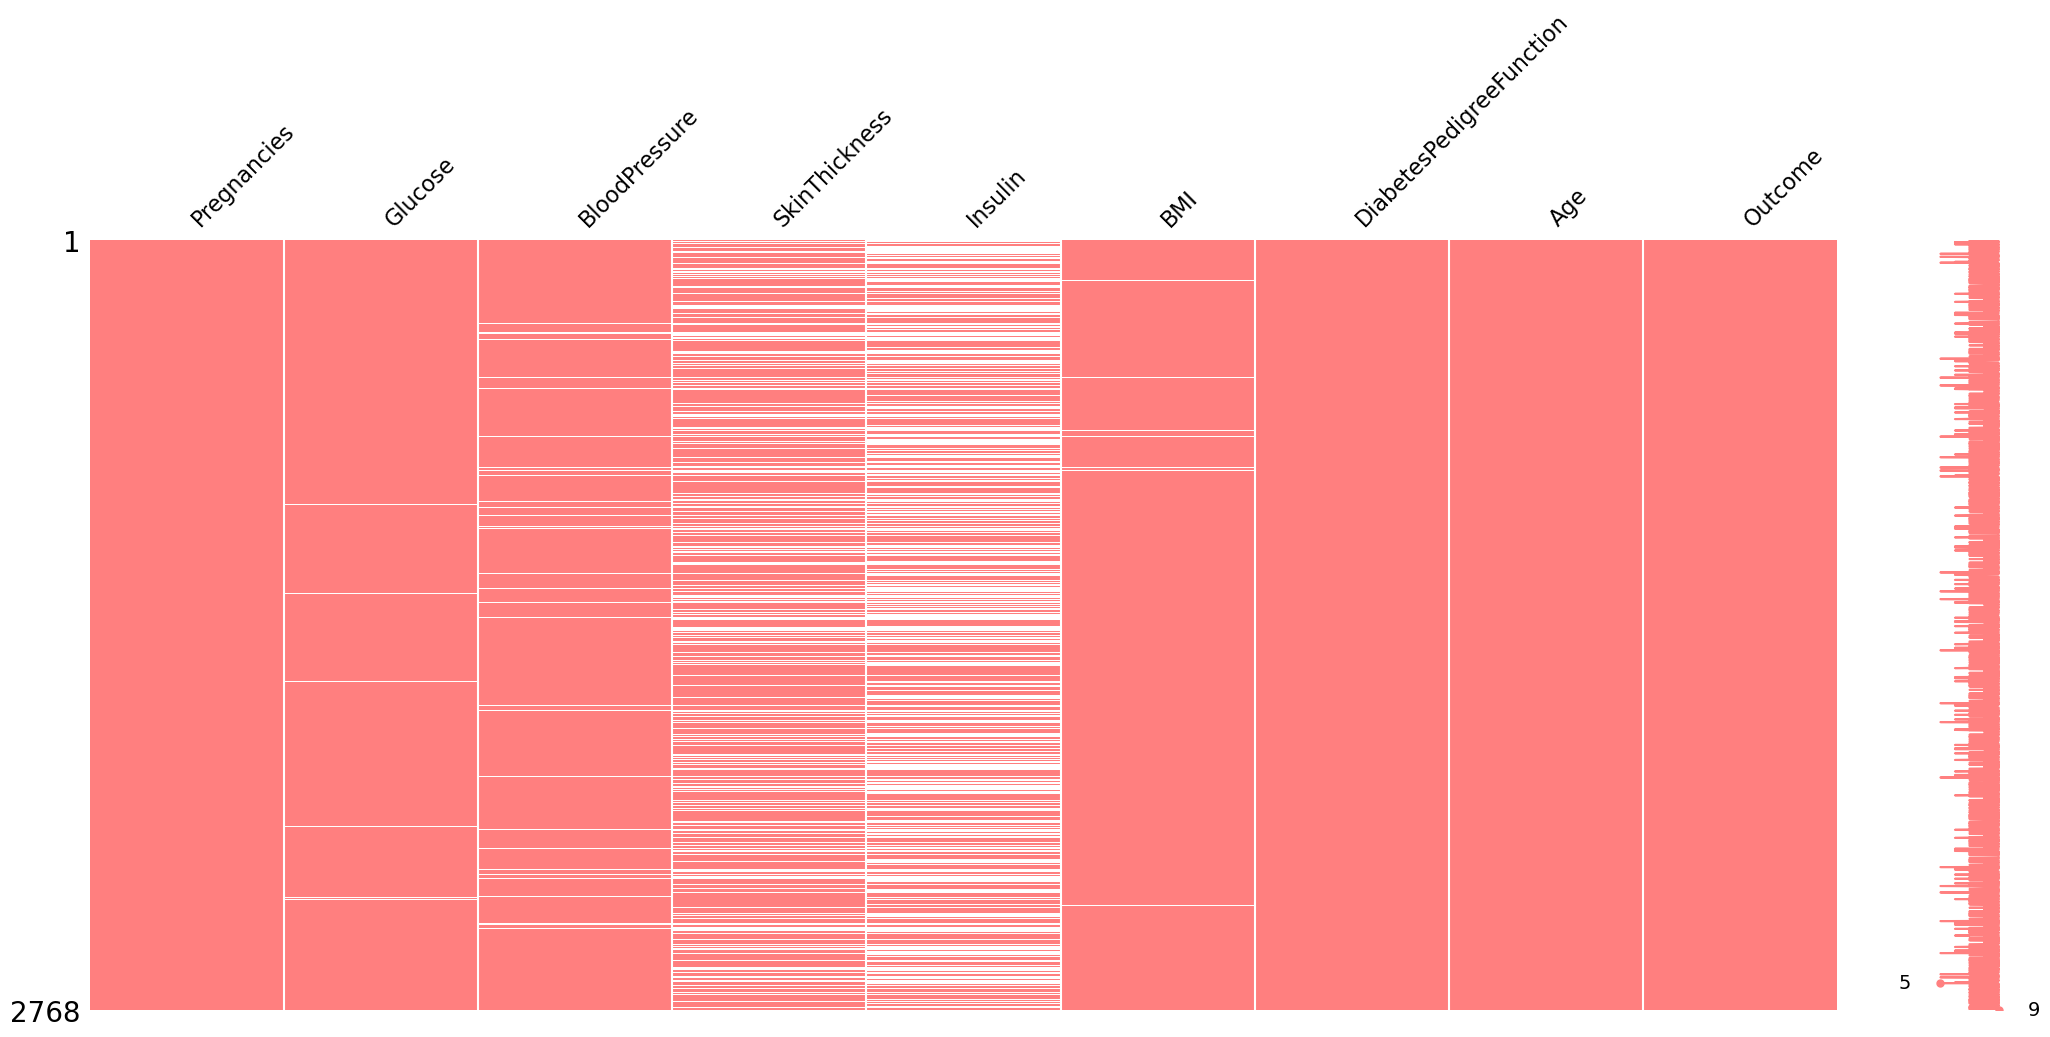
\includegraphics[width=\linewidth]{EDA/Plots/MissingnoMatrix.png}
    \caption{A Missingno matrix of the missing data per column.}
    \label{fig:MissingnoMatrix}
\end{figure}

% \begin{figure}[H]
%     \centering
%     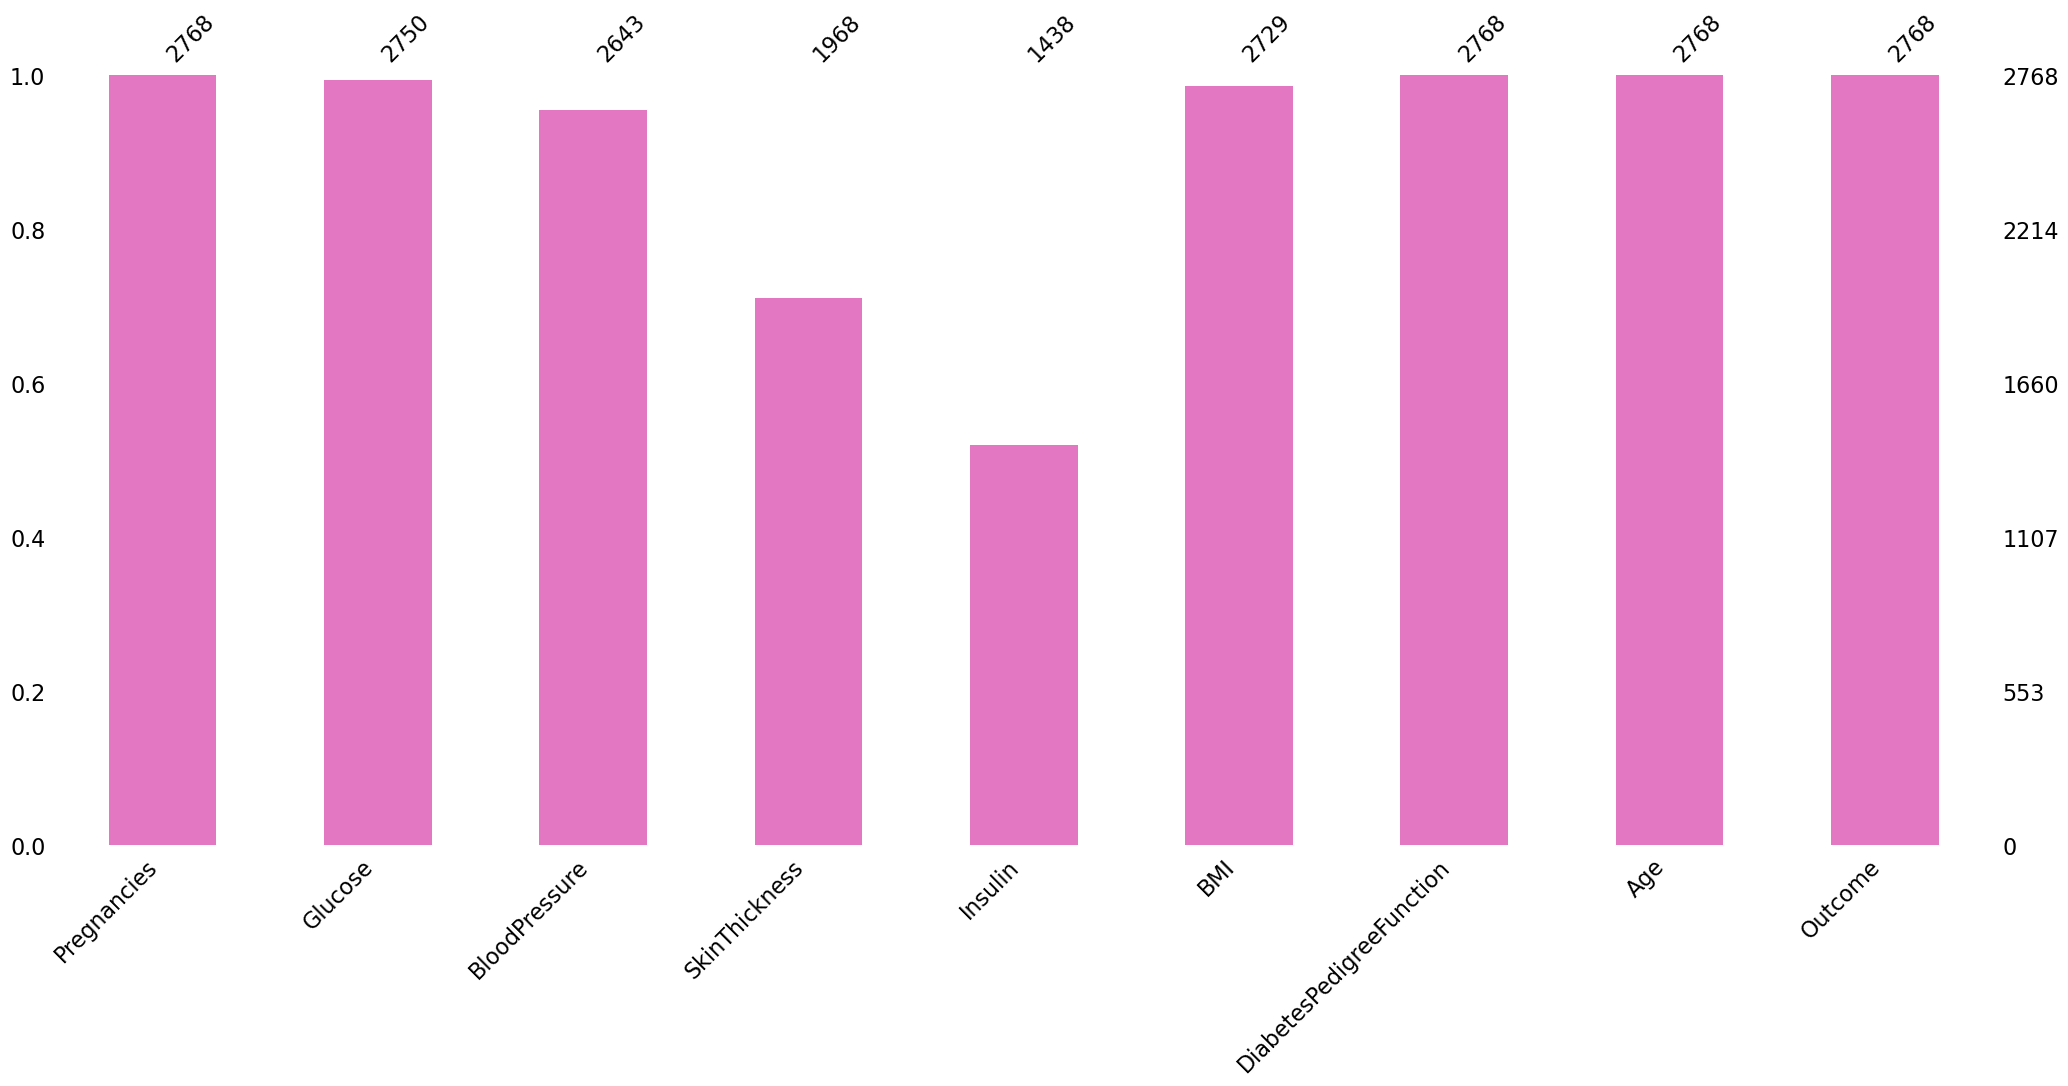
\includegraphics[width=\linewidth]{EDA/Plots/MissingnoBar.png}
%     \caption{A bar chart visualisation of the amount of data per column.}
%     \label{fig:MissingnoBar}
% \end{figure}

\para This matrix shows that the Insulin and SkinThickness columns contain considerable amounts of missing data alongside
many missing rows of BloodPressure, and some missing rows of BMI and Glucose, 
which will need to be fixed before any model can be trained. This is accomplished through imputation in Section 
\ref{sec:Preprocessing}.


\pagebreak 


\section{Target univariate analysis}\label{ASec:Imbalance}
Binary classification models can develop bias if they do not have enough data of both classes to accurately predict what combinations 
of values should determine each class. Therefore, it is essential to view the balance between classes as in Figure \ref{fig:ClassImbalancePlot}.

\begin{figure}[H]
    \centering
    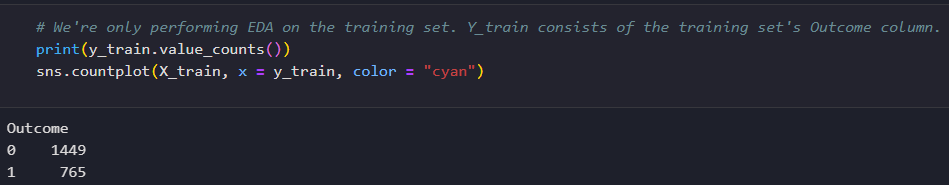
\includegraphics[width=.8\linewidth]{EDA/Code/TrainingValueCounts.png}
    \caption{The code to produce Figure \ref{fig:ClassImbalancePlot}.}
    \label{fig:ClassImbalancePlotCode}
\end{figure}

\begin{figure}[H]
    \centering
    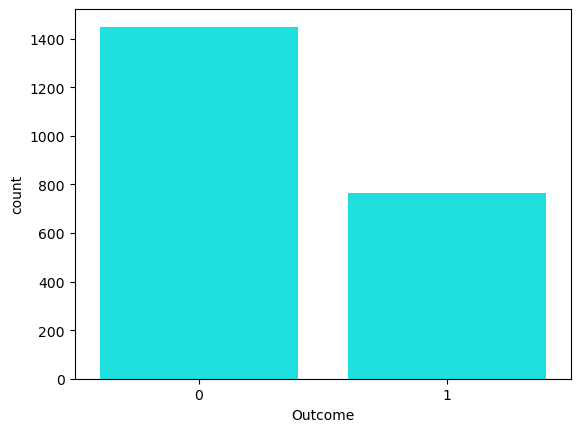
\includegraphics[width=.6\linewidth]{EDA/Plots/TrainingValueCounts.png}
    \caption{The class distribution of the training set (0: 1449, 1: 765).}
    \label{fig:ClassImbalancePlot}
\end{figure}

\para The dataset is imbalanced, favouring an outcome of 0. The exact percentages 
of each class can be calculated as seen below.

\begin{equation}
    \text{Outcome 0} = \frac{1449}{2214} = 0.655 \times 100\% = 65.5\%
\end{equation}

\begin{equation}
    \text{Outcome 1} = \frac{765}{2214} = 0.345 \times 100\% = 34.5\%
\end{equation}

\para The training set is 80\% of the data, hence why it is 2214 rows rather than 2768. From these calculations, it can be determined that 
there is an imbalance present in the training set, which will be resolved in Section \ref{sec:Preprocessing}.



\section{Multivariate analysis}
To compare each variable to each other and the outcome, the full training set previously  
created in Figure \ref{fig:FullTrainingSet} was used.

\subsection{Data distributions by Outcome}

It is important to identify significant outliers in the dataset so that models do not become skewed by the inflated variance, standard 
deviation and mean that they cause. Outliers that are very high in comparison to the primary distribution of the data will cause the 
standard deviation and mean to increase, whereas low outliers will make them decrease. Their identification is important not only for data analysis, 
but also for model development, as outliers can cause some algorithms to perform poorly or overfit, most notably distance-based algorithms 
such as K-Nearest Neighbours (KNN) and Support Vector Machines (SVM), which is further discussed in Section \ref{sec:ChosenAlgorithms}. 
% Source? It's true but cite something for that.

\para One of the simplest ways to visualise data distributions in the dataset is through box plots, which present the spread and skewness of numerical 
data in a simple visual format by showing the inter-quartile range (IQR). This has the added benefit of identifying outliers, as rows outside of the IQR. 
The boxplots of each column in the training set are shown below in Figure \ref{fig:AllBoxplotsByOutcome}. Each of the plots 
contains two boxplots, where one is for individuals without diabetes, and one is for those with diabetes.

\para In the figure, it can be seen that all columns contain some outliers.
However, most of these outliers are still relevant statistical data that would be possible, such as the outliers 
in Age being elderly people. Some of these outliers are less feasible, however; most notably the extreme high outliers 
in SkinThickness, BMI, and Insulin. Leaving these outliers in would affect the scaling of the data, and because it is generally 
ill-advised to remove rows of data especially with smaller datasets, they could instead be transformed to the upper bound to give 
a more even distribution. This will be accomplished in Section \ref{sec:Preprocessing}.

\begin{figure}[H]
    \centering
    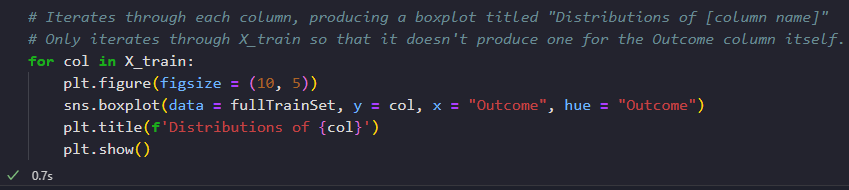
\includegraphics[width=\linewidth]{EDA/Code/BoxplotsByOutcome.png}
    \caption{The code used to produce Figure \ref{fig:AllBoxplotsByOutcome}.}
    \label{fig:BoxplotsByOutcomeCode}
\end{figure}


\begin{figure}[H]
    \centering
    % First row: 2 subfigures
    \begin{subfigure}[b]{0.45\textwidth}
        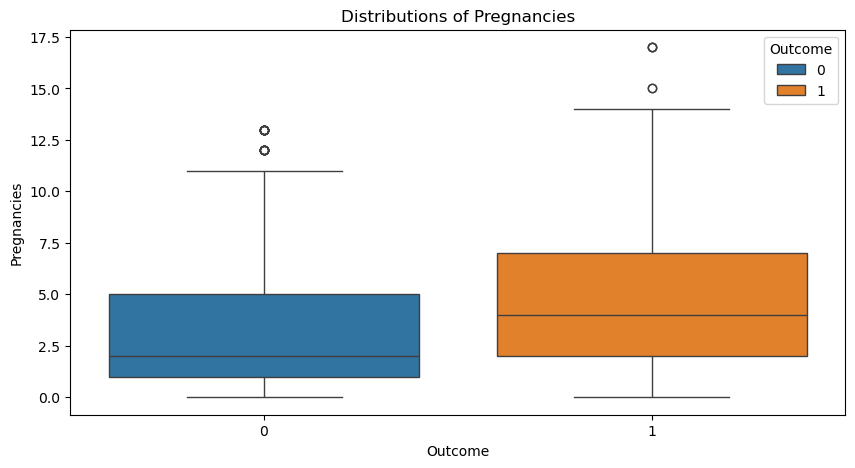
\includegraphics[width=\linewidth]{EDA/Plots/BoxplotsByOutcome/Pregnancies.png}
        \caption{Pregnancies}
        \label{fig:PregnanciesByOutcome}
    \end{subfigure}
    \hfill
    \begin{subfigure}[b]{0.45\textwidth}
        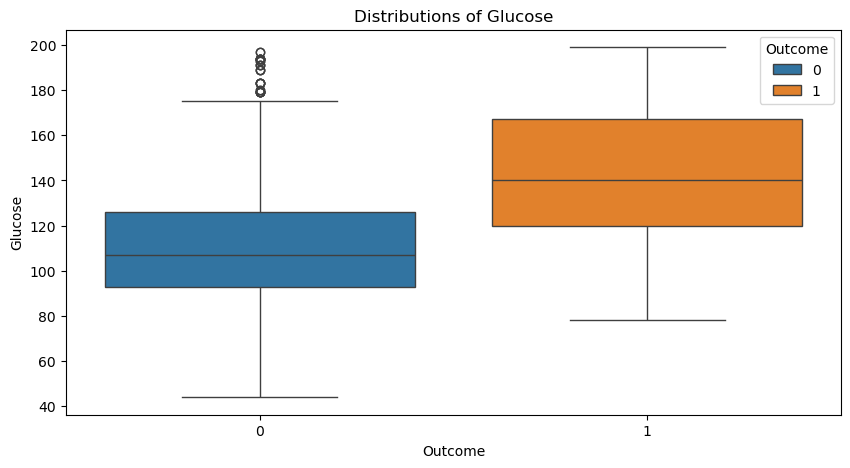
\includegraphics[width=\linewidth]{EDA/Plots/BoxplotsByOutcome/Glucose.png}
        \caption{Glucose}
        \label{fig:GlucoseByOutcome}
    \end{subfigure}
    
    \vspace{1em}
    
    % Second row: 2 subfigures
    \begin{subfigure}[b]{0.45\textwidth}
        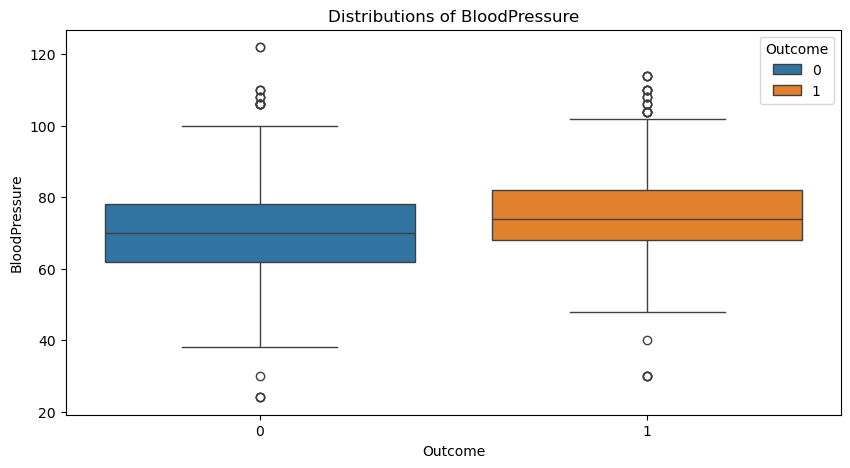
\includegraphics[width=\linewidth]{EDA/Plots/BoxplotsByOutcome/BloodPressure.png}
        \caption{BloodPressure}
        \label{fig:BloodPressureByOutcome}
    \end{subfigure}
    \hfill
    \begin{subfigure}[b]{0.45\textwidth}
        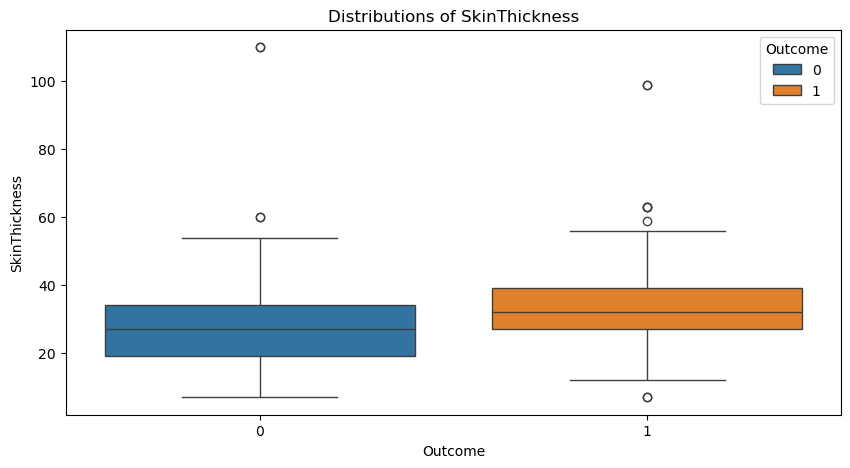
\includegraphics[width=\linewidth]{EDA/Plots/BoxplotsByOutcome/SkinThickness.png}
        \caption{SkinThickness}
        \label{fig:SkinThicknessByOutcome}
    \end{subfigure}
    
    \vspace{1em}
    
    % Third row: 2 subfigures
    \begin{subfigure}[b]{0.45\textwidth}
        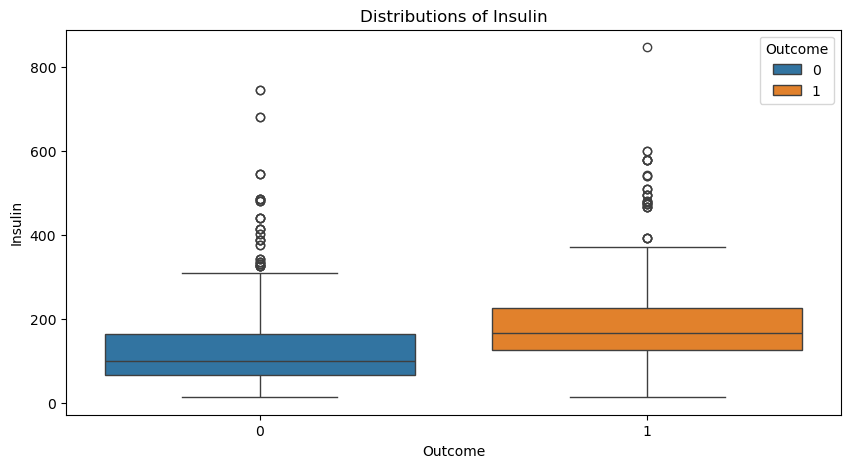
\includegraphics[width=\linewidth]{EDA/Plots/BoxplotsByOutcome/Insulin.png}
        \caption{Insulin}
        \label{fig:InsulinByOutcome}
    \end{subfigure}
    \hfill
    \begin{subfigure}[b]{0.45\textwidth}
        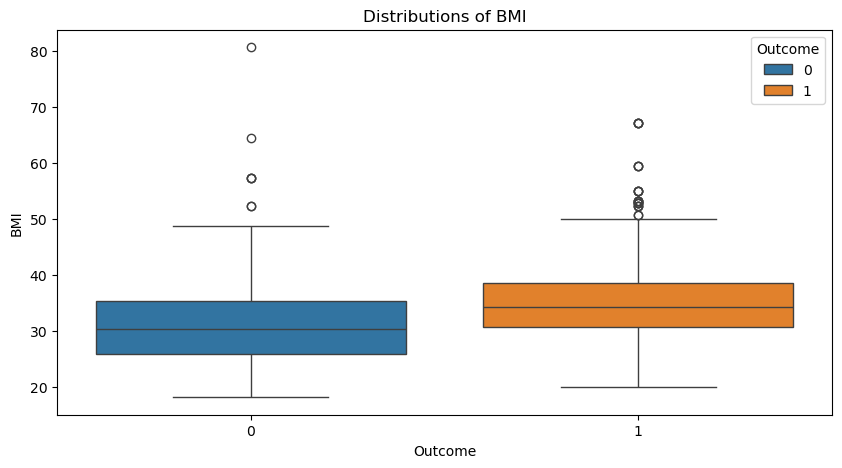
\includegraphics[width=\linewidth]{EDA/Plots/BoxplotsByOutcome/BMI.png}
        \caption{BMI}
        \label{fig:BMIByOutcome}
    \end{subfigure}
    
    \vspace{1em}
    
    % Fourth row: 2 subfigures
    \begin{subfigure}[b]{0.45\textwidth}
        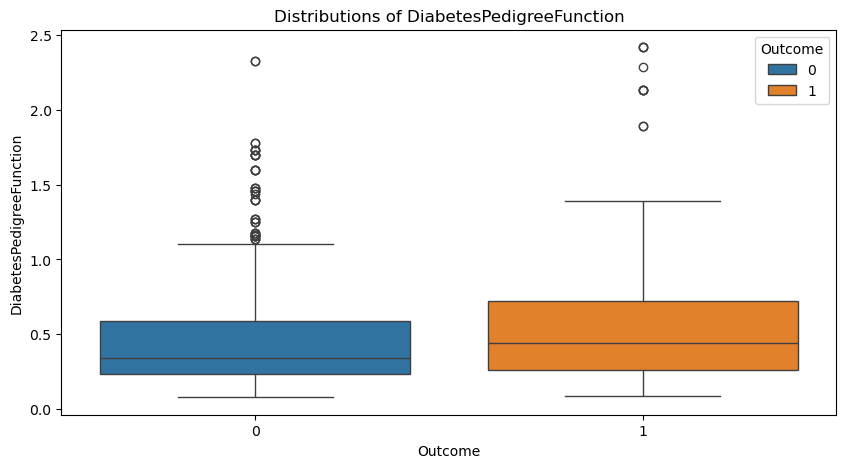
\includegraphics[width=\linewidth]{EDA/Plots/BoxplotsByOutcome/DiabetesPedigreeFunction.png}
        \caption{DiabetesPedigreeFunction}
        \label{fig:PedigreeByOutcome}
    \end{subfigure}
    \hfill
    \begin{subfigure}[b]{0.45\textwidth}
        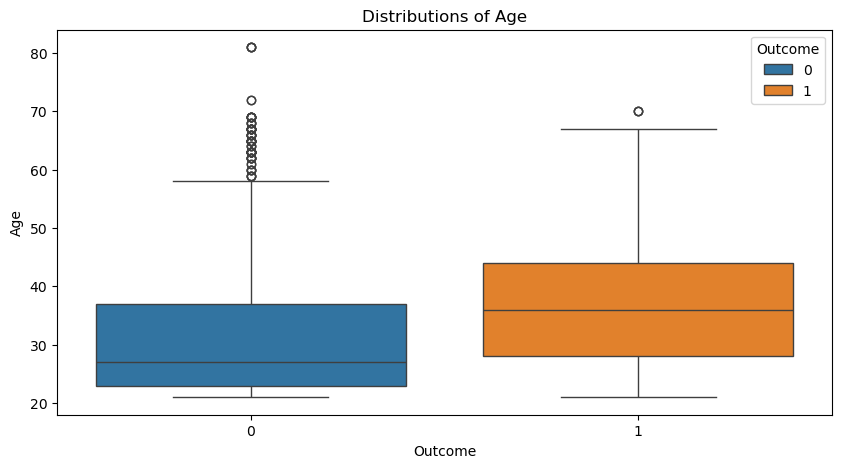
\includegraphics[width=\linewidth]{EDA/Plots/BoxplotsByOutcome/Age.png}
        \caption{Age}
        \label{fig:AgeByOutcome}
    \end{subfigure}
    
    \caption{Boxplots of all features by the outcome (Blue: No diabetes, Orange: Diabetes).}
    \label{fig:AllBoxplotsByOutcome}
\end{figure}

\pagebreak

\subsubsection{Pregnancies}
It was assumed in Table \ref{tab:Assumptions} that the amount of pregnancies a woman has had may bear a strong correlation
on whether they develop type 2 diabetes. This box plot does support the original assumption that the amount of pregnancies can positively 
correlate with the diabetes outcome, as the median and upper quartiles of the distributions of those with 
diabetes are higher than those without, though it also confirms that pregnancies are not a decisive factor 
on their own, as some patients had many pregnancies without having diabetes.

\subsubsection{Glucose}
This feature clearly shows a direct and strong correlation with the outcome; individuals with diabetes have
much higher glucose values, with a clear upward shift in both the median and interquartile range (IQR).
The lower whisker of the boxplots begins much higher with patients with diabetes, which implies that low glucose is a strong 
indicator that a patient does not have diabetes.

\subsubsection{BloodPressure}
Blood pressure values are fairly similar between the two groups, though individuals with diabetes show a slightly higher median.
Both groups have similar variability and range, indicating that blood pressure is not as strong a distinguishing factor. 
However, this slight correlation is still useful information, so this column should be kept. 

\subsubsection{SkinThickness}
This column contains significant outliers that will cause issues with data scaling.
Aside from these outliers, it does appear that skin thickness positively correlates with the outcome.

\subsubsection{Insulin}
This column contains many outliers, with some of these being extremely high. Aside from these, 
the main IQRs of the plots appear to indicate that higher insulin values are indicative of diabetes,
showing a positive correlation.

\subsubsection{BMI}
Individuals with diabetes tend to have higher BMI values on average.
The median BMI for the diabetic group is higher, with a slightly larger IQR, showing that BMI is an important factor in distinguishing diabetes outcomes.

\subsubsection{DiabetesPedigreeFunction}
The diabetes pedigree function has a slightly higher median for individuals with diabetes, but the difference is not substantial.
Both groups share significant overlap, suggesting that this feature alone may not strongly differentiate between outcomes, which 
differs from the original assumption.

\subsubsection{Age}
Individuals with diabetes tend to be older on average, as indicated by a higher median age for the diabetic group, and the fact that 
the IQR for the diabetic group is shifted upwards. However, many outliers without diabetes exist.


\para Another way to view data distributions is through histograms, which group data into "bins" before counting the occurrence of 
data in each bin and plotting this similarly to a bar plot. These are very useful for viewing the distribution curves of data. 
An additional feature of Seaborn is the Kernel Density Estimate (KDE), which will plot a line showing the distribution in the histogram.


\begin{figure}[H]
    \centering
    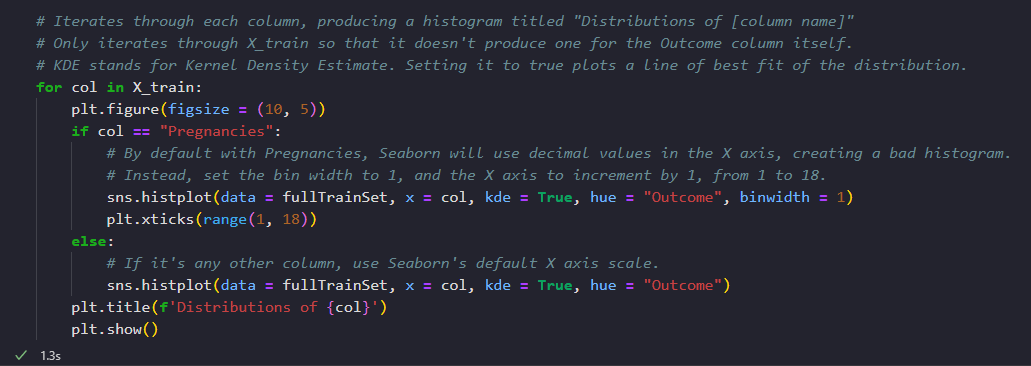
\includegraphics[width=\linewidth]{EDA/Code/HistogramsByOutcome.png}
    \caption{The code used to produce Figure \ref{fig:AllHistogramsByOutcome}.}
    \label{fig:HistogramsByOutcomeCode}
\end{figure}

\para Figure \ref{fig:AllHistogramsByOutcome} on the following page shows the distributions of each 
feature. There are a variety of distributions, with many features having left-skewed distribution curves,
though others such as BloodPressure and Glucose have bell curves, also known as normal distributions.
Interestingly, Age follows a power law distribution, with the vast majority of data inhabiting the lower 
values, which would correlate with the knowledge of the dataset - women aged 21 or over had data collected,
which reasonably explains why many of the values are from women aged between 20 and 30.

\begin{figure}[H]
    \centering
    % First row: 2 subfigures
    \begin{subfigure}[b]{0.45\textwidth}
        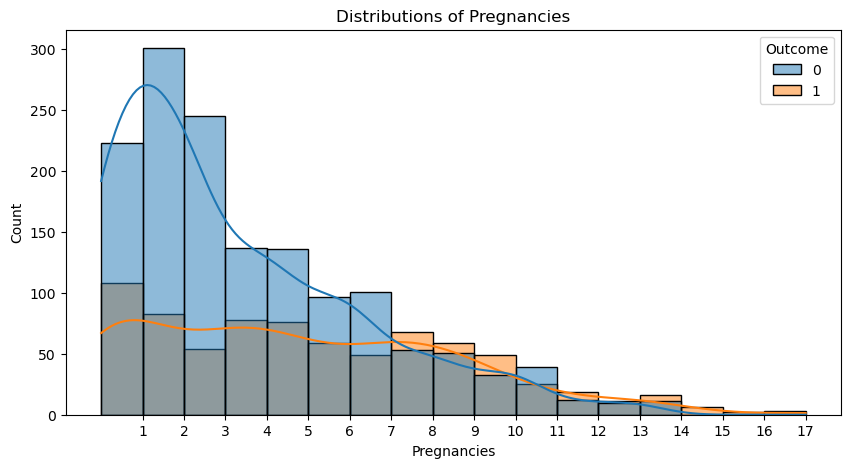
\includegraphics[width=\linewidth]{EDA/Plots/HistogramsByOutcome/Pregnancies.png}
        \caption{Pregnancies}
        \label{fig:PregnanciesByOutcomeHist}
    \end{subfigure}
    \hfill
    \begin{subfigure}[b]{0.45\textwidth}
        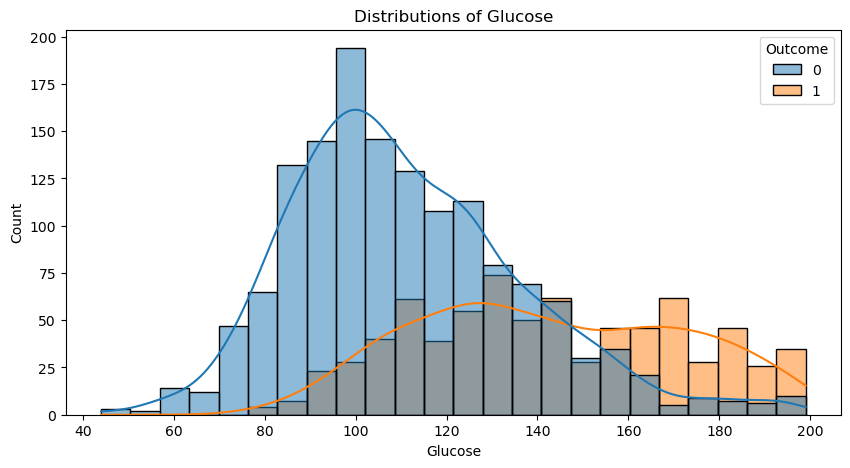
\includegraphics[width=\linewidth]{EDA/Plots/HistogramsByOutcome/Glucose.png}
        \caption{Glucose}
        \label{fig:GlucoseByOutcomeHist}
    \end{subfigure}
    
    \vspace{1em}
    
    % Second row: 2 subfigures
    \begin{subfigure}[b]{0.45\textwidth}
        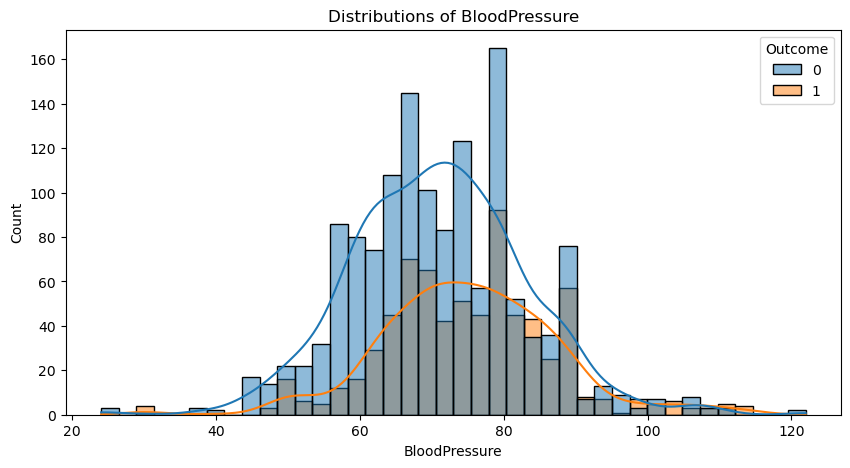
\includegraphics[width=\linewidth]{EDA/Plots/HistogramsByOutcome/BloodPressure.png}
        \caption{BloodPressure}
        \label{fig:BloodPressureByOutcomeHist}
    \end{subfigure}
    \hfill
    \begin{subfigure}[b]{0.45\textwidth}
        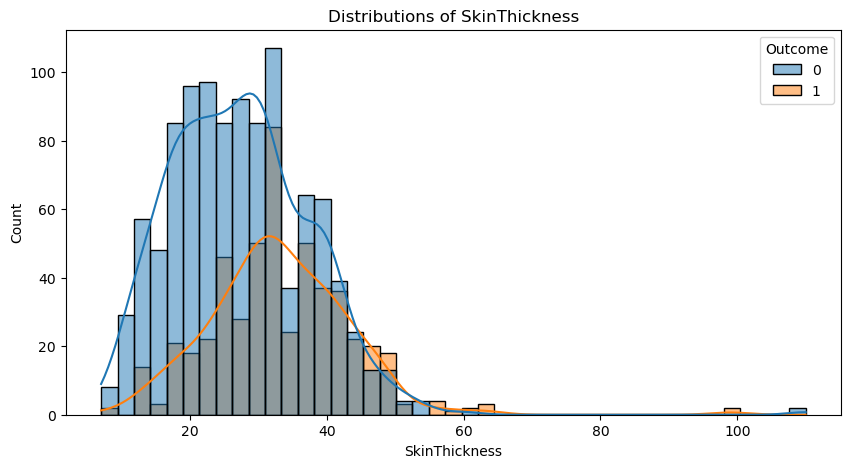
\includegraphics[width=\linewidth]{EDA/Plots/HistogramsByOutcome/SkinThickness.png}
        \caption{SkinThickness}
        \label{fig:SkinThicknessByOutcomeHist}
    \end{subfigure}
    
    \vspace{1em}
    
    % Third row: 2 subfigures
    \begin{subfigure}[b]{0.45\textwidth}
        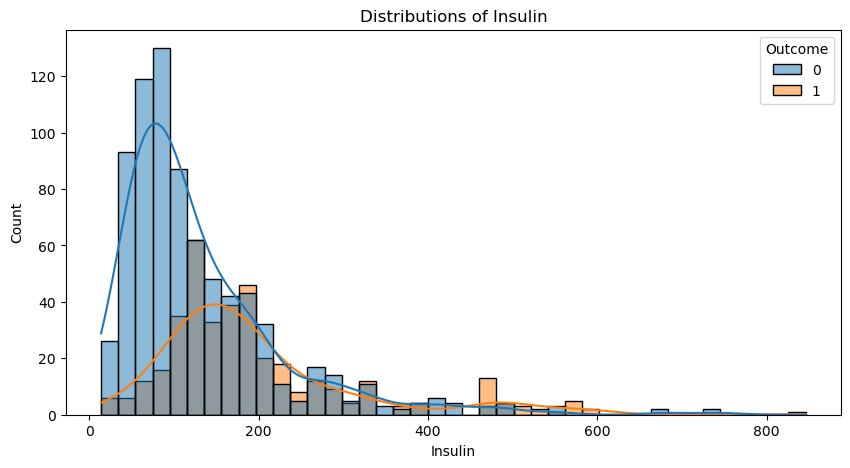
\includegraphics[width=\linewidth]{EDA/Plots/HistogramsByOutcome/Insulin.png}
        \caption{Insulin}
        \label{fig:InsulinByOutcomeHist}
    \end{subfigure}
    \hfill
    \begin{subfigure}[b]{0.45\textwidth}
        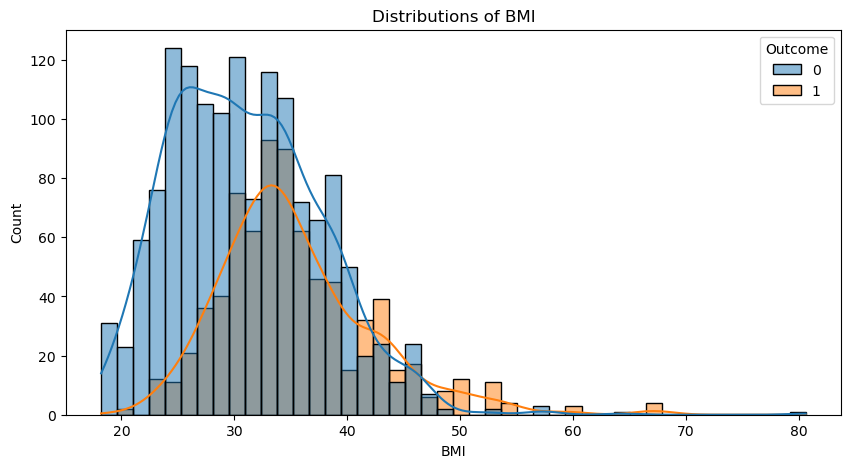
\includegraphics[width=\linewidth]{EDA/Plots/HistogramsByOutcome/BMI.png}
        \caption{BMI}
        \label{fig:BMIByOutcomeHist}
    \end{subfigure}
    
    \vspace{1em}
    
    % Fourth row: 2 subfigures
    \begin{subfigure}[b]{0.45\textwidth}
        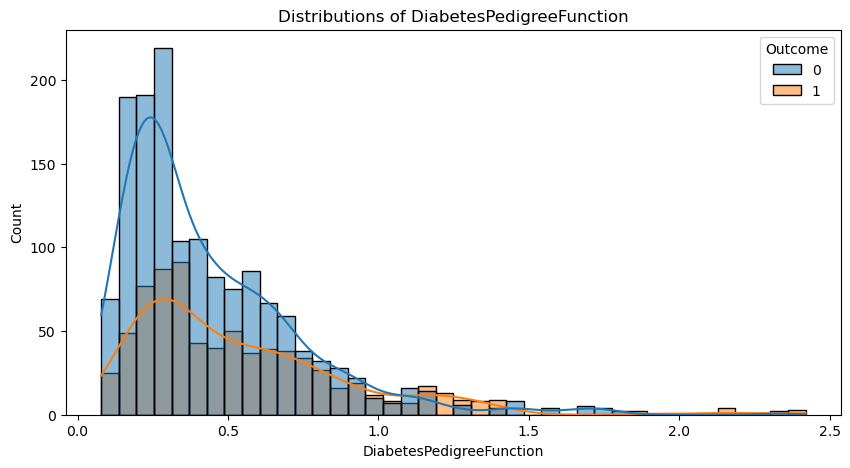
\includegraphics[width=\linewidth]{EDA/Plots/HistogramsByOutcome/DiabetesPedigreeFunction.png}
        \caption{DiabetesPedigreeFunction}
        \label{fig:PedigreeByOutcomeHist}
    \end{subfigure}
    \hfill
    \begin{subfigure}[b]{0.45\textwidth}
        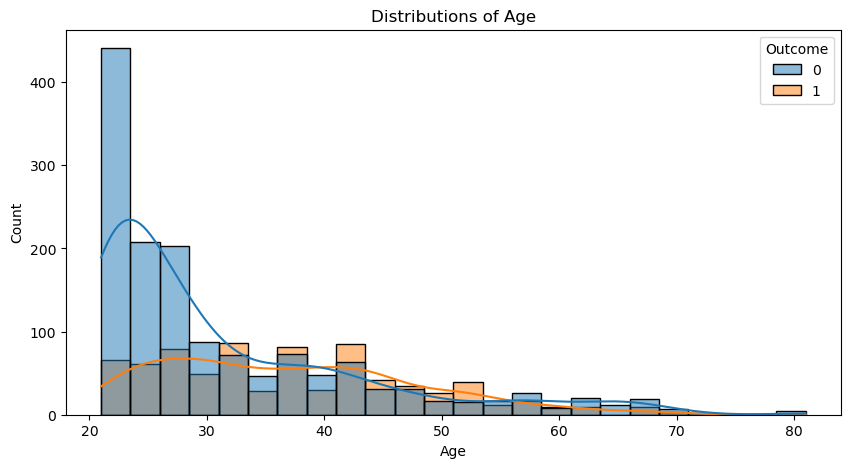
\includegraphics[width=\linewidth]{EDA/Plots/HistogramsByOutcome/Age.png}
        \caption{Age}
        \label{fig:AgeByOutcomeHist}
    \end{subfigure}
    
    \caption{Histograms of all features by the outcome (Blue: No diabetes, Orange: Diabetes).}
    \label{fig:AllHistogramsByOutcome}
\end{figure}


\subsection{Pair plot}
% This section is weak, though I don't know how best to improve it.
To view every column in the dataset plotted against each other, a pair plot can be created using Seaborn,
pictured in Figure \ref{fig:PairPlot}.

\begin{figure}[H]
    \centering
    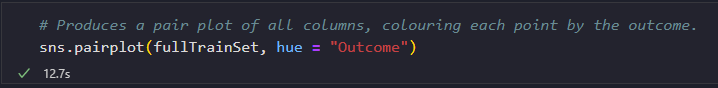
\includegraphics[width=\linewidth]{EDA/Code/PairPlot.png}
    \caption{The code to produce Figure \ref{fig:PairPlot}.}
    \label{fig:PairPlotCode}
\end{figure}

\begin{figure}[H]
    \centering
    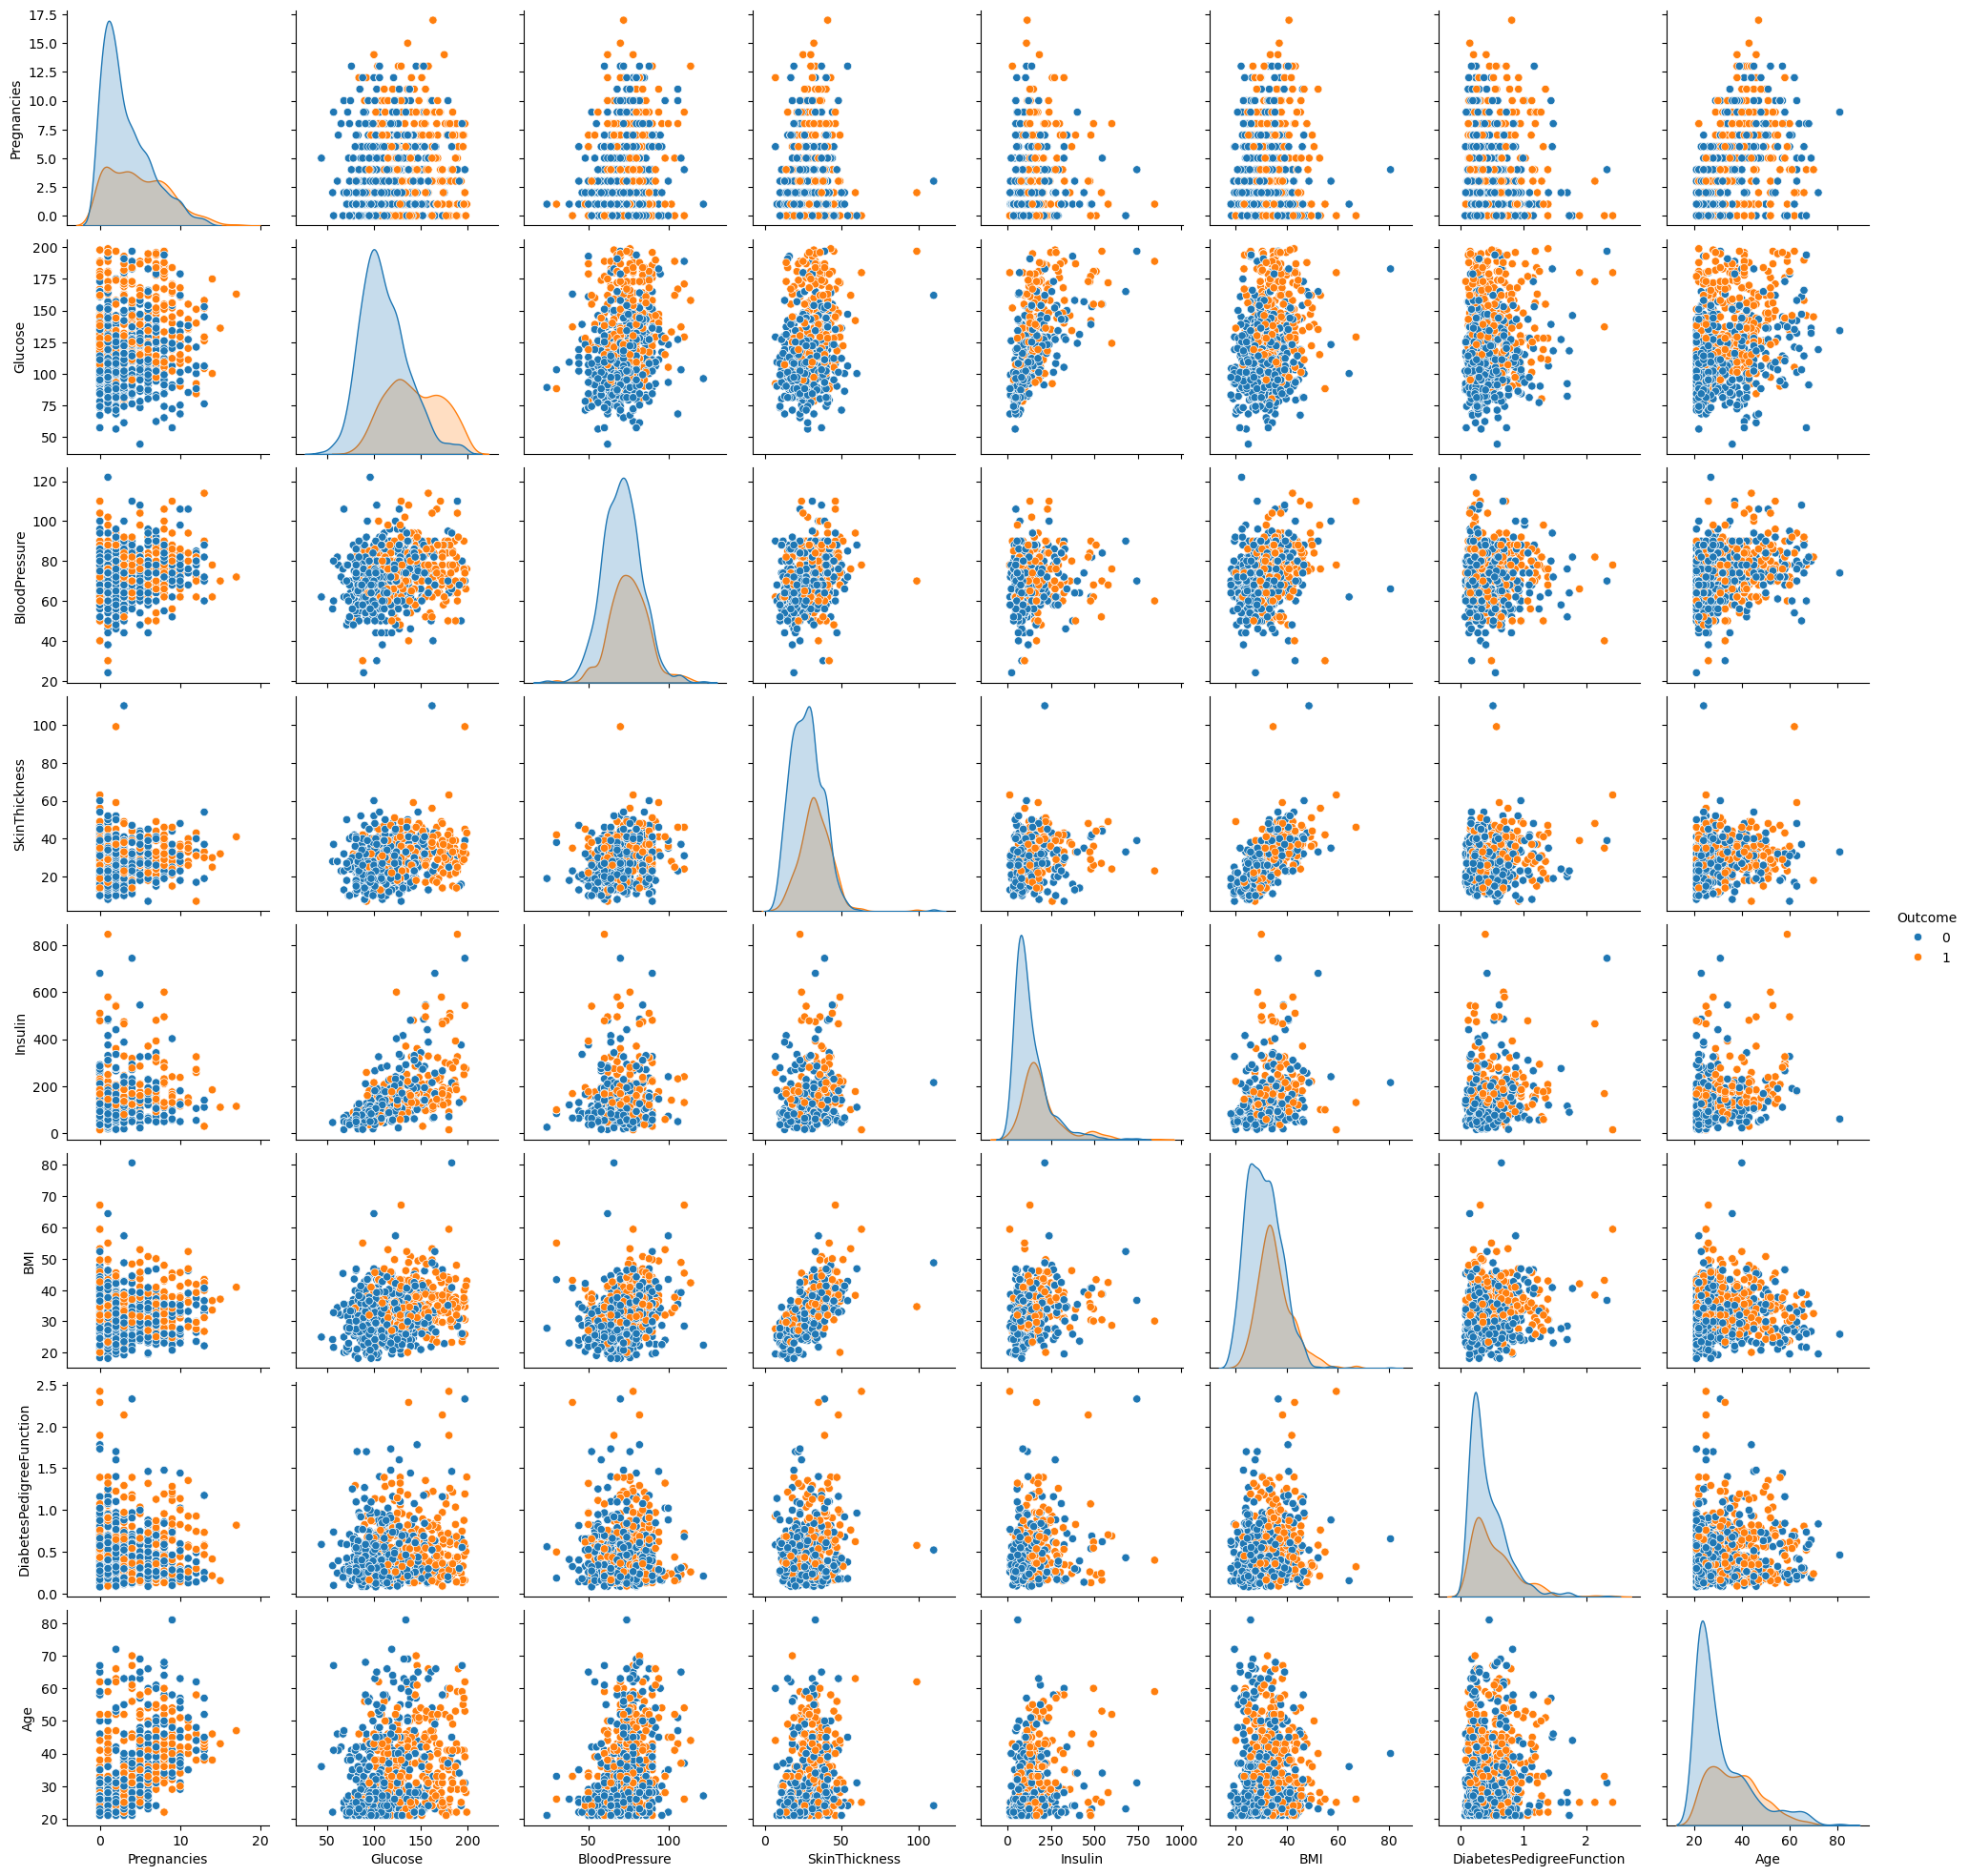
\includegraphics[width=\linewidth]{EDA/Plots/PairPlot.png}
    \caption{The pair plot of the full training set (Blue: No diabetes, Orange: Diabetes).}
    \label{fig:PairPlot}
\end{figure}

\para There are multiple observations on the relationships between features to be made from this pair plot, such as:
\begin{itemize}
    \item Glucose, BMI and Outcome 
        \begin{itemize}
            \item Glucose and BMI appear to be the two strongest predictors, with there being more cases of diabetes as each of these features increase,
            shown by the higher clustering of points. 
            \item Glucose also appears to slightly increase as BMI increases, suggesting a slight positive correlation between the two features. 
        \end{itemize}
    \item Pregnancies and Age
        \begin{itemize}
            \item As expected, pregnancies do typically increase with age. 
        \end{itemize}
    \item Pregnancies and Outcome
        \begin{itemize}
            \item There is no clear separation in the outcome based on pregnancies alone, suggesting it may not be a decisive factor.
        \end{itemize}
    \item Age
        \begin{itemize}
            \item While a person's age appears to not be directly relevant to them having diabetes, it instead appears that older individuals 
            instead typically have higher glucose levels and BMI, which are decisive factors.
        \end{itemize}
    \item Insulin
        \begin{itemize}
            \item Appears to be a good predictor, but not quite as much as glucose. Most rows where Insulin is between 400 and 600 are diabetic.
        \end{itemize}
    \item SkinThickness and BMI
        \begin{itemize}
            \item As expected, these two features are closely interlinked as seen by the mostly tight clustering between them in their associated plot.
        \end{itemize}
\end{itemize}

\subsubsection{Relation between Insulin and Glucose by Outcome}
A particular relation of note given the subject matter is the relation between insulin and glucose dependent on whether the 
individual has diabetes or not. Type 2 diabetes is characterised by insulin resistance and underproduction, meaning that lower insulin values are 
expected as glucose rises. Figure \ref{fig:ScatterInsulinGlucose} details this relation in patients with and without diabetes.

\begin{figure}[H]
    \centering
    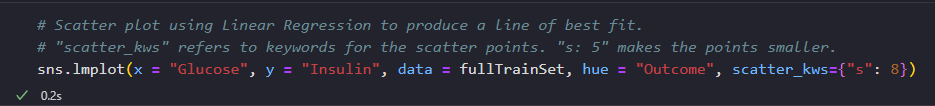
\includegraphics[width=\linewidth]{EDA/Code/ScatterInsulinGlucose.png}
    \caption{The code to produce Figure \ref{fig:ScatterInsulinGlucose}.}
    \label{fig:ScatterInsulinGlucoseCode}
\end{figure}

\begin{figure}[H]
    \centering
    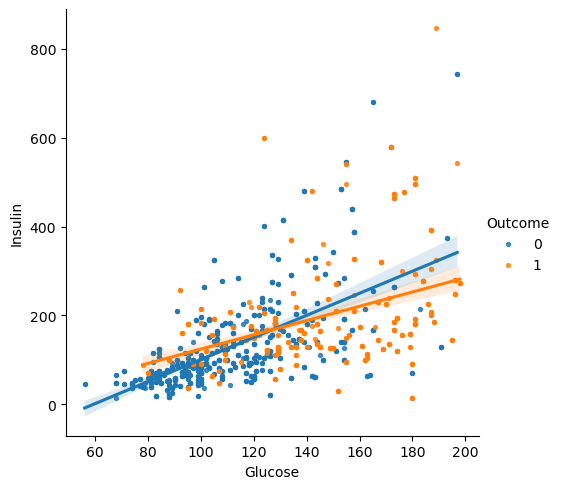
\includegraphics[width=\linewidth]{EDA/Plots/ScatterInsulinGlucose.png}
    \caption{A scatter plot with lines of best fit to show the trends in Insulin and Glucose.}
    \label{fig:ScatterInsulinGlucose}
\end{figure}

\para The expectation is matched, as glucose rises more than insulin in patients with diabetes, and slower 
than insulin in patients without diabetes.



\subsection{Correlation Matrix}
An alternative and simpler way to visualise the correlations between features in a dataset is through a correlation matrix as 
pictured in Figure \ref{fig:CorrMatrix}. The matrix uses the full training set created earlier to show the correlations between 
the dataset's features in an annotated heatmap format, quantifying each correlation as a number. Correlation matrices only work with numerical features, 
though all features are numeric in this dataset which enables the matrix to show all features. 

\begin{figure}[H]
    \centering
    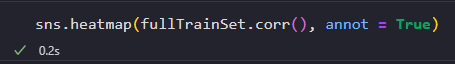
\includegraphics[width=\linewidth]{EDA/Code/CorrelationMatrix.png}
    \caption{The code to produce Figure \ref{fig:CorrMatrix}.}
    \label{fig:CorrMatrixCode}
\end{figure}

\begin{figure}[H]
    \centering
    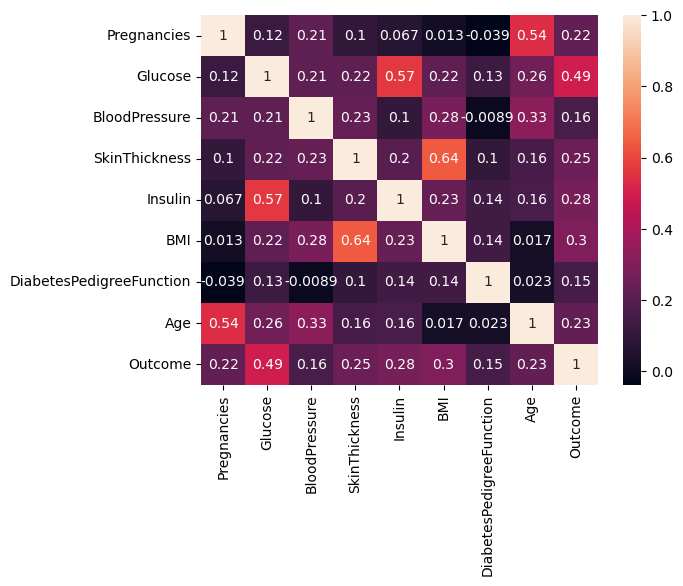
\includegraphics[width=\linewidth]{EDA/Plots/CorrelationMatrix.png}
    \caption{The correlation matrix of the full training set.}
    \label{fig:CorrMatrix}
\end{figure}

\para The correlation matrix reflects many of the observations noted in the pair plot and data distributions.
It shows the relationships between all features, including many expected relations like those of Glucose and Outcome,
Pregnancies and Age, and BMI and SkinThickness. However, the matrix also reveals insights that subvert the previous 
assumptions about the dataset, such as the pedigree function actually having the weakest correlation with the outcome.
This can be explained through other insights in the data as well as academic research.

\para \textcite{mambiya_play_2019} argue that diabetes mellitus can be caused by genetic predisposition, which is 
represented by the pedigree function in this dataset, though lifestyle factors such as weight gain and poor dietary 
variance can be a more significant factor in the cause of the disease in both those with and without genetic predispositions.
Their findings are also echoed within this dataset, with high BMIs representing overweightness/obesity and high Glucose values representing 
high sugar intake, which are the two most significant factors in the outcome according to the correlation matrix.

\endgroup
% Interesting trick to instead make the chapter number the letter B for this appendix.
\begingroup
\renewcommand\thechapter{B}
\titleformat{\chapter}[display]
{\normalfont\huge\bfseries}{}{20pt}{\Huge}
\setcounter{section}{0} % Set the section counter back to 0 so Appendix A doesn't interfere.

\chapter*{Appendix B - Classification Algorithms}
\addcontentsline{toc}{chapter}{Appendix B - Classification Algorithms}
\markboth{Appendix B}{}

\section{Random Forest}
Random forests are ensemble models, meaning that they leverage multiple other models and average their findings to 
give a single result. The other models used by a random forest are decision trees, which are flowchart-like structures where 
data is split at each node of the tree based on feature values to arrive at a classification. Random forests create many decision 
trees based on randomly sampling the dataset, and these trees then classify rows based on what they learn. Then, the predictions 
for each row by all decision trees are aggregated, and the prediction reached by the most trees is used.
The amount of decision trees used is a parameter that can be set, and the computational requirements of the algorithm 
also increase alongside this amount.
% This was written half-asleep at 12am and likely doesn't make much sense.

\para Random forests are reputed as one of the best classification algorithms, and are used frequently in many fields 
including diabetes diagnosis as seen in works from \textcite{chang_pima_2023} and \textcite{alzubi_diabetes_2023},
demonstrating their suitability for this classification task.
% They're resistant to overfitting, too. Talk about this.

\section{Support Vector Machine}
Support vector machines aim to find the optimal hyperplane\footnote{A decision boundary that separates the classes. In a two-dimensional graph, this would be a line of best fit, but in a multidimensional dataset, it would be a hyperplane.}
which separates classes with the highest possible margin, and are commonly used in classification problems \autocite{ibm_what_2023}. Data points on either 
side of the margin are known as support vectors. Figure \ref{fig:OptimalSVM} shows how a perfect SVM would look in a two-dimensional dataset for demonstrative purposes.

\begin{figure}[H]
    \centering
    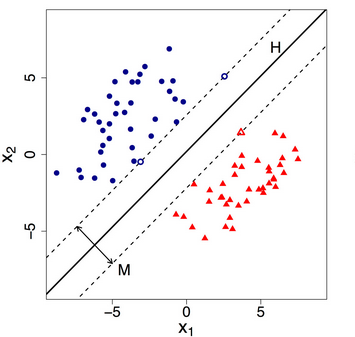
\includegraphics[width=.5\linewidth]{Algorithms/OptimalSVM.png}
    \caption{An optimal SVM that demonstrates the algorithm's key features. Rows on the dotted line are the support vectors, the solid line is the hyperplane, and the space
    between the hyperplane and support vectors is the margin. \autocite{kirchner_using_2018}}
    \label{fig:OptimalSVM}
\end{figure}

\para \textcite{kirchner_using_2018} state that SVMs are computationally intensive, requiring lots of memory and processing power 
to run optimally. Additionally, \textcite{atla_sensitivity_2011} mention that SVMs are particularly sensitive to noise in 
datasets, meaning their quality can be poor when there are many outliers. Despite these drawbacks, however, they can still 
be useful in diabetes classification as observed in the work of \textcite{zou_construction_2024}.

\section{Logistic Regression}
Logistic regression computes a weighted sum of all input features, where the appropriate weights are learned by the algorithm as it trains.
A sigmoid function, shown in Equation \ref{eq:Sigmoid}, is then used to transform the sum to a value between 0 and 1, which is then used to classify the row as 0 if it is below 
0.5, or classify it as 1 if it is above 0.5. 

\begin{equation}\label{eq:Sigmoid}
    f(x) = \frac{1}{1 + e^{-x}}     
\end{equation}

\para Logistic regression is a very common algorithm in binary classification tasks, as it is simple to implement and interpret, and
can perform well even with limited amounts of training data \autocite{kavya_applications_2024}. It has also been widely used in previous 
analyses of the Pima Indian dataset. (\textcite{alzubi_diabetes_2023}, \textcite{joshi_predicting_2021}, \textcite{zou_construction_2024})

\section{Na\"ive Bayes}
Na\"ive Bayes is an example of a probabilistic classification algorithm \autocite{ibm_what_2021}, as it is based on Bayes' theorem,
which calculates the probability of an event given that another event has occurred, shown in Equation \ref{eq:Bayes}. 
In binary classification, it is the probability of the target given the other features. Na\"ive Bayes gets its name from its na\"ive assumption
that features are all independent of each other.

\begin{equation}\label{eq:Bayes}
    P(A|B) = \frac{P(B|A) \cdot P(A)}{P(B)}
\end{equation}

\para This theorem calculates that the probability of an event occurring is equal to the probability of the event given 
prior knowledge multiplied by the prior probability of the event. This can be contextualised to this specific dataset, shown in Equation \ref{eq:ContextBayes}.

\begin{equation}\label{eq:ContextBayes}
    P(Diabetes | Other features) = \frac{P(Other features | Diabetes) \cdot P(Diabetes)}{P(Other features)}
\end{equation}

\para Gaussian Na\"ive Bayes is used in this project, as it is best suited to continuous data as seen in this dataset's 
features. Interestingly, Na\"ive Bayes typically has lower accuracy than other models such as Random Forests \autocite{khan_novel_2023},
though it has been used in previous diabetes classification tasks \autocite{aftab_cloud-based_2021, chang_pima_2023, zou_construction_2024}.

\section{K-Nearest Neighbours (KNN)}
The k-Nearest Neighbours (kNN) algorithm is a fundamental machine learning classification method that operates by identifying 
the $k$ closest training examples to a data point across all features and assigns the most common class among these neighbours 
as the prediction. $K$ is a parameter that can be set within the algorithm, and has a heavy influence over its accuracy.
KNN doesn't make any assumptions about the distribution of the data, making it useful for complex, real-world scenarios
such as healthcare \autocite{thomas_addressing_2021}, and has also been used on the Pima Indian and Frankfurt datasets
to high success \autocite{alzubi_diabetes_2023, zou_construction_2024}.


% Interesting trick to instead make the chapter number the letter C for this appendix.
\begingroup
\renewcommand\thechapter{C}
\titleformat{\chapter}[display]
{\normalfont\huge\bfseries}{}{20pt}{\Huge}
\setcounter{section}{0} % Set the section counter back to 0 so that Appendix B doesn't interfere.

\chapter*{Appendix C - What is data encoding?}
\addcontentsline{toc}{chapter}{Appendix C - What is data encoding?}
\markboth{Appendix C}{}

Machine learning models are unable to directly interpret string data. This is a significant issue 
in many datasets, as some features may contain strings for categorical data, such as "Yes" and "No", for example.
To solve this issue, data is \textbf{encoded} to a numerical representation. Many strategies exist to do so,
for both nominal and ordinal data.

\section{Nominal data}
Nominal data is defined by \textcite{oxford_brookes_university_types_nodate} as "unordered, categorical 
and mutually exclusive", providing examples of country names or "Yes" or "No" questions\footnote{Data with only two possibilities is known as dichotomous data \autocite{oxford_brookes_university_types_nodate}.}.
Mutually exclusive means that data cannot fit into multiple of these categories, as a question cannot be answered with both "Yes" and 
"No", for example. To encode nominal data, processes such as one-hot encoding are used.

\subsection{One-hot encoding}
One-hot encoding is a technique to encode nominal data by creating new features representing each possibility of the data.
For example, if a "Countries" feature included "England", "America", and "France", one-hot encoding of that feature would 
replace the original feature with "Countries\_England", "Countries\_America", and "Countries\_France", where the data in each of these 
would either be a 1 or 0 based on what the row's value originally was. With one-hot encoding, it is especially important to ensure 
data does all fit in the expected categories, as errors like spelling mistakes would cause the creation of an entirely new and 
irrelevant feature.

\para Because a new feature is created for every possibility, one-hot encoding drastically increases the dimensionality of 
datasets it is leveraged against. This can massively increase storage and processing requirements, especially in datasets 
with many rows.

\section{Ordinal data}
\textcite{oxford_brookes_university_types_nodate} defines ordinal data as "ordered, categorical and mutually exclusive."
The examples they provide are BMI categories (underweight, normal, overweight, obese) and questionnaire answers (strongly disagree,
disagree, etc.). Ordinal data can be encoded using processes such as label encoding.

\subsection{Label encoding}
Label encoding encodes ordinal data by assigning integer values to each possibility. Reusing the questionnaire example, "strongly disagree"
could correlate to 1, with "disagree" correlating to 2, and so on\footnote{This particular example is known as a "Likert scale". \autocite{oxford_brookes_university_types_nodate}}. 
Encoding data in this way maintains its ordinal nature, as machine learning algorithms can interpret "larger number = better", which allows them
to use the data for classification or regression tasks. 

\para If label encoding is used on non-ordinal data, however, it can mislead machine learning algorithms into believing there is an inherent 
order in data where there is not, and interpret these as relationships that do not exist. Reusing the countries example, if data such 
as "England", "America" and "France" was encoded to 1, 2 and 3 respectively, a machine learning algorithm may interpret France as being the 
best country, despite them all being equal. 

\printbibliography

\end{document}